\documentclass[utf8]{gradu3}
% Jos työ on kandidaatintutkielma eikä pro gradu, käytä ylläolevan asemesta
%\documentclass[utf8,bachelor]{gradu3}
% Jos kirjoitat englanniksi, käytä ylläolevan asemesta
%\documentclass[utf8,english]{gradu3}
% tai
%\documentclass[utf8,bachelor,english]{gradu3}

\usepackage{graphicx} % kuvien mukaan ottamista varten
\graphicspath{ {./kuvat/} }

\usepackage{amsmath} % hyödyllinen jos tekstisi sisältää matikkaa,
                     % ei pakollinen

\usepackage{booktabs} % hyvä kauniiden taulukoiden tekemiseen

\usepackage{float}
\usepackage{changepage}
\usepackage{geometry}

\usepackage{xcolor}
\definecolor{darkred}{HTML}{820d00}

% HUOM! Tämän tulee olla viimeinen \usepackage koko dokumentissa!
\usepackage[bookmarksopen,bookmarksnumbered,linktocpage]{hyperref}
\hypersetup{
    colorlinks=true,
    linkcolor=blue,
    citecolor=darkred,
    filecolor=magenta,      
    urlcolor=cyan,
}

\addbibresource{gradu.bib} % Lähdetietokannan tiedostonimi

\begin{document}

\title{Äänipalautetyökalun suunnittelu, toteutus ja evaluointi}
\translatedtitle{Design, implementation and evaluation of recorded audio feedback -tool}
\studyline{Ohjelmistotekniikka}
\avainsanat{%
  suunnittelututkimus, äänipalaute, työkalu, audio-ohjelmisto, palautemuoto, heuristiikat, oppimisympäristö
  }
\keywords{design science, recorded audio feedback, tool, audio-software, feedback form, heuristics, virtual learning environment}
\tiivistelma{%
Palaute on yksi merkittävimpiä yksittäisiä tekijöitä oppimisen kannalta, ja sen tulisi olla   ajankohtaista, ymmärrettävää ja oppilaan hyödynnettävissä.  Aänipalaute on todettu tehokkaaksi palautemuodoksi tekstimuotoisen palautteen ohella, ja sen suosio on kasvanut opetuskäytössä vuosien varrella. Se on muun muassa yksityiskohtaisempaa, ymmärrettävempää ja henkilökohtaisempaa kuin tekstimuotoinen palaute, sekä suhtautuminen sitä kohtaan on yleisesti positiivista, niin opettajien kuin oppilaidenkin keskuudessa. Äänipalautteen antaminen koostuu palautteen nauhoittamisesta ja sen jakamisesta, ja nämä toimenpiteet voidaan suorittaa useilla eri tavoilla. Tässä tukimuksessa suunniteltiin ja toteutettiin äänipalautteen antamiseen suunnattu web-pohjainen työkalu, jota evaluoimalla selvitettiin, voidaanko äänipalautteen antamista helpottaa entisestään tai voidaanko suhtautumista sen antamiseen muuttaa. Työkalun suunnittelussa ja toteutuksessa hyödynnettiin Nielsenin heuristiikkoja ja Gestaltin hahmolakeja, joilla voidaan perustella käyttöliittymiä koskevia valintoja. Osaan ratkaisuista päädyttiin yhteistyössä pro gradu -ohjaajien kanssa, joista molemmat ovat hyödyntäneet äänipalautetta omassa opetuksessaan. Tavoitteena oli luoda mahdollisimman helppokäyttöinen työkalu, joka sisältää ainoastaan äänipalautteen antamisen kannalta oleelliset toiminnot, jotta oppimiskynnys sen käyttöön olisi mahdollisimman matala. Työkalu toteutettiin responsiivisena web-sovelluksena, jotta sen käyttö onnistuisi laitteesta riippumatta ilman erillistä asennusta. Työkalun evaluointi suoritettiin kahdessa iteraatiossa, joista ensimmäiseen osallistui kaksi koehenkilöä. Ensimmäisen evaluoinnin pohjalta työkaluun tehtiin parannuksia ja lisäominaisuuksia, jonka jälkeen suoritettiin toinen evaluointi neljän koehenkilön toimesta. Kahden evaluoinnin tulosten perusteella voidaan sanoa, että tutkimuksessa onnistuttiin löytämään  sellaisia suunnitteluratkaisuja, jotka testihenkilöt kokivat helpottaviksi äänipalautteenannon kannalta. Helpottavia tekijöitä oli toiminnallisuuksien vähäinen määrä, käyttöliittymän yksinkertaisuus ja selkeys, Insert-Record toiminto, sekä joustavuus.  Testihenkilöiden suhtautuminen äänipalautteen antamiseen ei sen sijaan muuttunut työkalun käytön muuta, sillä he suhtautuivat siihen jo alunperin positiivisesti.  
}
\abstract{%
  ...
}

\author{Erkko Mäkinen}
\contactinformation{\texttt{erkko.e.makinen@student.jyu.fi}}
% jos useita tekijöitä, anna useampi \author-komento
\supervisor{Anneli Heimbürger ja Ville Isomöttönen}
% jos useita ohjaajia, anna useampi \supervisor-komento

%\type{Tietotekniikan pro gradu -tutkielma} % et tarvitse tätä riviä tutkielmassa!

\maketitle

%\begin{thetermlist}
%\item[RAF] Recorded audio feedback \parencite[ks.][]{using}. 
%\end{thetermlist}

\mainmatter

\chapter{Johdanto}

Palautteenanto on erittäin tärkeä osa opetusta. Sen perusteella opiskelijat tietävät, missä asioissa he ovat suoriutuneet hyvin, ja missä heillä on vielä kehitettävää. Se voidaan suorittaa useilla eri tavoilla, ja siinä voidaan hyödyntää erilaisia palautemuotoja, joilla jokaisella on omat hyvät ja huonot puolensa. Äänipalautteen (engl. Recorded Audio Feedback, RAF) hyödyntäminen opetuskäytössä on yleistynyt viime vuosina, ja sen hyödyt on havaittu erityisesti verkko-opetuksen parissa, jossa suoraa kontaktia opettajaan tai muihin opiskelijoihin ei välttämättä ole lainkaan. Se on validi palautemuoto tekstimuotoisen palautteen ohella, ja opiskelun muuttuessa vuosi vuodelta yhä teknologia-avusteisemmaksi, on tilanteeseen mukauduttava myös palautteenannon osalta, jotta palautteenanto olisi mahdollisimman tehokasta, niin opettajille kuin oppilaillekin.

Tämänhetkisten tutkimusten perusteella äänipalaute koetaan yleisesti positiivisena sekä opettajien että oppilaiden keskuudessa. Äänipalaute pystytään antamaan nopeasti, se on tekstimuotoista yksityiskohtaisempaa ja selkeämpää, sekä asiat voidaan käsitellä keskustelunomaisesti vaikeasti ymmärrettävän akateemisen kielen sijaan \parencite{developing}. Lisäksi äänensävyllä voidaan korostaa ja helpottaa palautteen tulkitsemista, ja palautteen kuuleminen lukemisen sijaan tuntuu henkilökohtaisemmalta, mikä vaikuttaa positiivisesti oppimiseen \parencite{attitudes}. Heimbürgerin, Isomöttösen, Kedon ja Niemisen \parencite*{academics} mukaan äänipalaute toimii parhaiten täydentävänä tai vaihtoehtoisena palautemuotona tekstimuotoisen palautteen ohella, ja se soveltuu erityisesti kirjoitustehtäviin. He kuitenkin tuovat ilmi, että tarkkuutta vaativiin tehtäviin soveltuu paremmin tekstimuotoinen palaute \parencite{academics}. Opiskelijoiden mukaan äänipalaute tukee oppimista parhaiten siten, että palautteen pääkohdat kirjataan tiiviisti tekstimuotoisena sähköpostiin ja yksityiskohtaisemmat perustelut niitä koskien äänipalautteeseen \parencite{using}.

Vaikka äänipalautteella on tutkittu olevan selkeitä etuja tekstimuotoiseen palautteeseen nähden tietyillä osa-alueilla, sen asettamat tekniset vaatimukset voivat johtaa jopa palautemuodon poissulkemiseen \parencite{developing}. Äänipalautteen nauhoittaminen ja jakaminen voidaan suorittaa useilla eri työkaluilla ja alustoilla, mutta perinteiset audio-ohjelmistot sisältävät usein runsaasti erilaisia toiminnallisuuksia, jotka voivat vaikeuttaa niiden oppimista ja käyttämistä. Toisaalta osa työkaluista mahdollistaa ainoastaan palautteen nauhoittamisen, muttei sen editoimista, jolloin virheen sattuessa nauhoitusprosessi on aloitettava alusta. On otettava huomioon, että alkuvaiheessa erilaiset tekniset esteet vaikuttavat negatiivisesti äänipalautteen antamiseen kokemuksena \parencite{versus}, joten tarvetta helppokäyttöiselle työkalulle, jolla myös vähäiset tietotekniset taidot omaavat opettajat pystyvät nauhoittamaan, editoimaan ja jakamaan palautteensa, löytyy varmasti. Äänipalautteen antoon suunnattu työkalu saattaa parhaimmassa tapauksessa jopa lisätä äänipalautteen antamista, jolloin yhä useampi oppilaista pääsee hyötymään kyseisestä palautemuodosta omassa oppimisessaan.

Tämän suunnittelututkimuksen tavoitteena on suunnitella, kehittää ja evaluoida äänipalautteen antamiseen tarkoitettu työkalu, joka mahdollistaa äänileikkeiden nauhoittamisen ja editoimisen mahdollisimman helposti. Pro gradu -tutkimuksen laajuus ei riitä kokoversion toteuttamiseen työkalusta, joten siitä luodaan prototyyppi, jonka suunnittelun ja kehityksen aikana pyritään kartoittamaan erilaisia tarpeita äänipalautteen antamiseen liittyen. Prototyypin painopisteet ovat tarkoituksenmukasuudessa, helppokäyttöisyydessä ja käytettävyydessä, jotta äänipalautteen antaminen työkalua hyödyntäen olisi mahdollisimman intuitiivista ja mutkatonta. 

Tutkimus suoritetaan kahdessa iteraatiossa, jotka koostuvat työkalun suunnittelusta, kehityksestä ja iteraation päättävistä evaluoinneista.  Pääpaino iteraation eri vaiheista on evaluoinneissa, joissa testihenkilöt käyttävät äänipalautetyökalua simuloidusti autenttisessa tilanteessa, ja vastaavat työkalun eri osa-alueita koskeviin kysymyksiin kyselylomakkeella. Testihenkilöt kuuluvat informaatioteknologian alan opetushenkilökuntaan, ja kullakin heistä on aiempaa kokemusta äänipalautteen antamisesta, joten he pystyvät vertaamaan työkalun käyttöä aiempiin kokemuksiinsa. Evaluoinnin tuloksia analysoimalla tavoitteena on vastata kahteen tutkimuskysymykseen:

\begin{itemize}
  \item Helpottaako äänipalautetyökalu äänipalautteen antamista entuudestaan?
  \item Muuttaako äänipalautetyökalun käyttö suhtautumista äänipalautteen antamiseen?
\end{itemize}

Luvussa 2 käsitellään palautteenantoa ja äänipalautetta yleisellä tasolla, sen hyviä ja huonoja puolia, sekä äänipalautteen antamista opettajan näkökulmasta. Luvussa 2 käydään läpi tarkemmin suunnittelututkimuksen eri vaiheita, ja tutkimuksen toteutusta peilaten valintoja suunnittelututkimuksen periaatteisiin. Luvussa 3 käsitellään äänipalautetyökalun toteutusta, teknisiä toteutusratkaisuja, suunnitteluun vaikuttaneita käytettävyysheuristiikkoja, käyttöliittymää sekä työkalun erikois- ja perustoimintoja. Luku 4 koostuu kahden iteraation tuloksista ja niiden pohjalta laadituista jatkotoimenpiteistä. Luku 5 sisältää pohdintaa tutkimuksen tuloksista, potentiaalisista jatkotutkimuksen aiheista, sekä tutkimuksen onnistumisesta kokonaisuudessaan. 

\chapter{Äänipalaute}

\section{Yleistä palautteenannosta ja äänipalautteesta}

Palautteenanto on tärkeä osa arviointiprosessia, ja sen vaikutusta voidaan pitää yksittäisistä tekijöistä merkittävimpänä oppimisen edistäjänä \parencite{gibbs2004}. Palaute voi olla joko formatiivista tai summatiivista, riippuen arvioinnin funktiosta. Formatiivinen arviointi suoritetaan oppimisen aikana, ja sen tarkoituksena on arvioida, kuinka hyvin mitkäkin asiat on opittu, ja missä asioissa on vielä parantamisen varaa. Summatiivinen arviointi taas suoritetaan oppimisen jälkeen, ja oppilaan osaamisen tasoa verrataan siihen, mitä hänen tulisi osata tietyn standardin mukaan \parencite{biggs2011}. Palautteenannossa erityisen tärkeää on palautteen tehokkuus, jotta oppimista tapahtuisi mahdollisimman paljon. Gibbsin ja Simpsonin \parencite*{gibbs2004} mukaan tehokkaan palautteen tulisi olla ymmärrettävää ja ajanakohtaista, sekä oppilaan tulisi pystyä hyödyntämään sitä tulevissa opinnoissaan. Palautteenantoon liittyy kuitenkin tiettyjä haasteita, jotka ovat Biggsin ym. \parencite*{biggs2011} mukaan havaittavissa oppilaiden tyytymättömyytenä palautteeseen globaalilla tasolla, useiden eri tutkimusten pohjalta. Lisäksi, koska palautteenannossa on kaksi osapuolta, oppilas ei välttämättä tulkitse palautetta opettajan tarkoittamalla tavalla, mikä on ongelmallista \parencite{sadler2010}. Edellä mainituista syistä palautteenannon sekä erilaisten palautemuotojen ja niiden välisten suhteiden tarkempi tutkiminen on merkittävää. 

Äänipalaute (engl. Recorded Audio Feedback) voidaan määritellä tätä nykyä digitaaliseksi äänitiedostoksi, joka sisältää formatiivisen tai summatiivisen verbaalisen palautteen ohjaajalta oppilaalle \parencite{developing}. Äänipalaute ei kuitenkaan ole uusi palautemuoto, sillä sitä on hyödynnetty jo kasettinauhureiden aikakautena etäopetuksessa, tosin pienimuotoisesti teknologisten rajoitteiden vuoksi \parencite{developing}. Teknologiaa hyödynnetään opetuskäytössä yhä enemmän ja enemmän, ja useiden tutkimusten mukaan sen avulla voidaan tehostaa palautteenantoa usein eri tavoin. Se esimerkiksi tarjoaa oppilaille joustavuutta, sillä digitaaliseen palautteeseen voi perehtyä haluamanaan ajankohtana omassa rauhassa, ja sen hyödyntäminen myös myöhempinä ajankohtina onnistuu helposti, kun taas esimerkiksi kirjallinen palaute voi vahingoittua tai kadota \parencite{technology}. Oppilasmäärien kasvaminen sekä verkko-opetuksen laajempi hyödyntäminen tuo toisaalta uusia haasteita opetukseen, sillä opettajien ja oppilaiden välinen suora kontakti vähenee entisestään \parencite{engaging}. Äänipalaute koetaan henkilökohtaisempana kuin tekstimuotoinen palaute \parencite{evaluating}, joten sen hyödyntäminen voi olla yksi keino oppilaan ja opettajan välisen kuilun kaventajana. Teknologian kehittymisen ansiosta myös koulutus on kansainvälisempää kuin ennen, joten kulttuurilliset erot on otettava opetuksessa huomioon. Heimbürgerin ja Isomöttösen \parencite*{moderating} mukaan äänipalautteen avulla saatetaan myös pystyä hillitsemään kulttuurillisten ulottuvuuksien vaikutuksia, mutta aihe vaatii vielä tarkempaa jatkotutkimusta.

Teknologisesta kehityksestä huolimatta äänipalaute ei ole kovin laajamittaisessa käytössä, vaikka useiden tutkimusten mukaan se on validi palautemuoto \parencite{engaging}. Vuonna 2008, palautteenantoa koskevan tutkimuksen mukaan, 85\% tutkimukseen osallistuvista opettajista antoi palautteensa tekstimuotoisena \parencite{electronic}. Osuus voi olla hieman eri tämän tutkimuksen tekohetkellä, mutta oletus on silti, että suurin osa palautteesta annetaan oppilaille edelleen tekstimuotoisena. Palautteenantoa kasvotusten pidetään tehokkaimpana keinona oppimisen kannalta, mutta se on erittäin työlästä, ja oppilas ei välttämättä muista kaikkia keskustelussa käytyjä asioita \parencite{modes}. Äänipalaute on palautemuoto, joka sijoittuu tekstimuotoisen ja kasvokkain tapahtuvan palautteenannon välille, yhdistellen näiden molempien palautemuotojen ominaisuuksia. Seuraavassa kappaleessa käsittellään tarkemmin äänipalautteen hyviä ja huonoja puolia sekä opettajan että oppilaan näkökulmista.

Useiden tutkimusten mukaan äänipalaute soveltuu parhaiten kirjoitustehtäviin \parencite{academics, engaging, using}, kun taas tarkkuutta vaativaan palautteeseen, kuten esimerkiksi matemaattiikka- ja ohjelmointitehtäviin, soveltuu paremmin tekstimuotoinen palaute, sillä informaatio voidaan ilmaista kirjoitettuna täsmällisemmin \parencite{academics}. Äänipalautteen soveltuvuuteen vaikuttaa tehtävätyypin lisäksi myös opiskelijan koulutustaso ja edistyminen opinnoissa. Heimbürgerin \parencite*{using} mukaan äänipalaute soveltuu parhaiten maisteri- ja tohtoriopiskelijoille, joilla akateemisen opiskelun perusteet ovat jo hallussa. Hennessyn ja Forresterin \parencite*{developing} mukaan äänipalaute taas soveltuu sekä opintojen alkuvaiheessa oleville että valmistuville, mutta sen antamisessa on otettava huomioon opintojen taso, sillä eri vaiheissa olevat opiskelijat suhtautuvat äänipalautteeseen eri tavoin.

Äänipalautetta voidaan hyödyntää useisiin eri tarkoituksiin, ja Heimbürger \parencite*{using} jaottelee äänipalautteen Sternin ja Salmonin \parencite*{stern} kategorisointia hyödyntäen globaalin-, keski-, mikro- ja meta-tason äänipalautteeseen. Äänipalautteen on havaittu keskittyvän usein arvioitavan tehtävän globaaleihin seikkoihin, kun taas kirjoitettu palaute sisältää usein mikro-tasoista, eli kielioppia ja oikeinkirjoitusta koskevaa palautetta \parencite{versus}. Tekstimuotoista palautetta pidetäänkin äänipalautetta tehokkaampana vaihtoehtona mikro-tasoisessa palautteenannossa \parencite{ice}. Eri palautetasojen lisäksi on oleellista mihin asioihin opettaja palautteessa keskittyy, ja mitä hän tuo siinä ilmi. Merry ja Osmond \parencite*{attitudes} havaitsivat, että äänipalaute sisältää enemmän oppimista tukevia kommentteja, kun taas tekstimuotoinen palaute sisältää enemmän sellaisia huomioita, jotka eivät ole oppimisen kannalta merkittäviä.

Tutkimustulokset osoittavat, että äänipalaute toimii parhaiten täydentävänä tai vaihtoehtoisena palautemuotona, esimerkiksi tekstimuotoisen palautteen ohella \parencite{academics, modes, ice}. Useiden palautemuotojen hyödyntäminen on kannattavaa myös siitä syystä, että näin voidaan välttää yksittäisen palautemuodon puutteellisuudet ja tehdä palautteenannosta mahdollisimman tehokasta ja mielekästä \parencite{modes}. Lisäksi oppilailla on laaja skaala erilaisia oppimistyylejä- ja preferenssejä, minkä vuoksi erilaisten palautemuotojen hyödyntäminen opetuksessa voi olla kannattavaa \parencite{style}. Palautemuotoa valitessaan opettajan tulisi kuitenkin huomioida erilaiset rajoitteet, kuten oppilaiden mahdolliset kuulo- tai näkövammat \parencite{evaluating}.

\section{Äänipalautteen hyviä ja huonoja puolia}

Äänipalautteella on useita hyötyjä tekstimuotoiseen palautteeseen nähden, ja yleinen suhtautuminen sitä kohtaan on positiivista sekä opettajien että oppilaiden keskuudessa. Yksi äänipalautteen merkittävimmistä eduista on se, että palaute on puhuttuna yksityiskohtaisempaa kuin kirjoitettuna, sillä se sisältää usein enemmän informaatiota \parencite{attitudes}. Äänipalaute on myös selkeää ja helposti ymmärrettävää, sillä asiat voidaan ilmaista keskustelunomaisesti, jolloin akateemisen kielen ja monimutkaisen sanaston käyttäminen on vähäisempää. Tekstimuotoisen palautteen ymmärrettävyyteen vaikuttavat negatiivisesti usein myös käsinkirjoituksesta johtuvat epäselvyydet tai huono käsiala, jotka voivat hidastaa palautteen tulkitsemista huomattavasti \parencite{developing}.

Äänenkäytöllä on palautteen yksityiskohtaisuuden ja ymmärrettävyyden lisäksi monia muita positiivisia vaikutuksia. Oppilaat kokevat äänipalautteen henkilökohtaisemmaksi, kuin tekstimuotoisen palautteen, mikä on merkittävä etu erityisesti etäopetuksessa, jossa oppilailla ei ole mahdollisuutta kasvotusten tapahtuvaan vuorovaikutukseen opettajan kanssa \parencite{using, distanceLearning}. Lisäksi oppilaat kokevat, että opettaja on nähnyt enemmän vaivaa äänipalautteen eteen, ja osaavat arvostaa sitä eri tavalla kuin tekstimuotoista palautetta \parencite{listenOrToRead}. Äänensävyllä on myös selvä vaikutus äänipalautteen tulkitsemiseen, sillä se esimerkiksi helpottaa palautteen ymmärtämistä, ja auttaa sisäistämään siitä kaikista tärkeimmän asiat \parencite{attitudes}. Heimbürgerin ja Isomöttösen \parencite*{moderating} toteuttaman tutkimuksen mukaan enemmistö äänipalautetta vastaanottavista opiskelijoista tahtoi palautteissaan käytettävän henkilökohtaista äänensävyä, joka sisältää runsaasti erilaisia nyansseja, muodollisen tai neutraalin äänensävyn sijaan. Äänenkäyttöön liittyy kuitenkin myös tiettyjä ristiriitoja sekä opettajien että oppilaiden osalta. Cavanaughin ja Songin \parencite{versus} toteuttamassa tutkimuksessa eräs opettaja koki kritiikin antamisen helpommaksi, sillä kritiikin pystyi perustelemaan paremmin, mutta toisaalta Heimbürgerin ym. \parencite*{academics} toteuttamassa tutkimuksessa eräs opettajista koki kritiikin antamisen töykeäksi, ja tästä syystä halusi nähdä oppilaan kasvotusten ennen palautemuodon hyödyntämistä. Myös osa oppilaista kokee kritiikin vastaanottamisen epämiellyttävänä, mutta kyse on selkeästä vähemmistöstä \parencite{voice}. 

Palautteen vastaanottaminen äänitteenä koetaan mielenkiintoisemmaksi ja miellyttävämmäksi kuin palautteen lukemisen tekstimutoisena \parencite{listenOrToRead}. Merryn ja Osmordin \parencite*{attitudes} toteuttaman tutkimuksen mukaan enemmistö opiskelijoista kuunteli äänipalautteen useammin kuin kerran, tehden alkuperäiseen tehtävään muutoksia palautetta kuunnellessaan, mikä merkitsee formatiivisen oppimisprosessin toteutumista. Myös Hennesyn ja Forresterin \parencite*{attitudes} mukaan oppilaat kuuntelivat äänipalautteen todennäköisemmin useaan kertaan, mutta edellä mainitusta tutkimuksesta poiketen osa oppilaista ei ollut mielissään formatiivisesta palautteesta aiheutuvasta lisätyöstä. Äänipalautteella on havaittu myös muita positiivisia vaikutuksia oppilaiden käytökseen, kuten se, että oppilaat palaavat todennäköisemmin äänipalautteen pariin suoriutuakseen myöhemmässä tehtävässä paremmin \parencite{voice}.

Yksi äänipalautteen merkittävä eduista opettajan näkökulmasta on se, että palautteen ilmaiseminen puhuttuna on nopeampaa kuin kirjoitettuna. Luntin ja Curranin \parencite*{areYouListening} mukaan minuutti puhetta vastaa noin kuutta minuuttia kirjoittamista, mikä on merkittävä ero ajansäästön kannalta. Suurin osa kirjallisuudesta tukee tätä väitettä, mutta mukaan mahtuu myös poikkeuksia. Esimerkiksi Cannin \parencite*{engaging} sekä Cavanaughin ja Songin \parencite*{versus} mukaan äänipalautteen antaminen säästää aikaa ainoastaan, kun sitä käytetään tekstimuotoisten kommenttien korvaajana. On otettava kuitenkin huomioon, että äänipalautteen antaminen on aluksi hitaampaa, jos opettajalla ei ole aiempaa kokemusta sen hyödyntämisestä opetuksessaan. Heimbürgerin ym. \parencite*{academics} toteuttamassa tutkimuksessa opettajilta kului aluksi äänipalautteen antamiseen enemmän aikaa kuin tekstimuotoiseen palautteenantoon, mutta lopulta prosessin opittuaan aikaa säästyi jopa 50\%, ja opettajat kokivat, että kognitiivinen ja fyysinen kuormitus väheni entuudestaan. Alkuvaiheen teknologiset haasteet voivatkin olla yksi syy siihen, että äänipalaute ei ole saavuttanut niin suurta suosiota kuin mihin sillä olisi potentiaalia. Äänipalautteen antamisessa on kuitenkin otettava huomioon se, että vaikka palautteen nauhoittaminen olisi helppoa ja nopeaa, palautteen jakaminen oppilaille voi olla aikaa vievää riippuen käytettävästä menetelmistä \parencite{engaging}.

Äänipalautteen yksi tunnetuista rajoitteista on visuaalisuuden puute, josta aiheutuu tiettyjä haasteita. Palautteesta voi olla vaikea hahmottaa mihin tehtävän ongelmaan palautteenantaja milläkin hetkellä viittaa \parencite{versus}, ja palautteen tiettyihin seikkoihin palaaminen myöhempinä ajankohtina vaatii palautteen kuuntelemisen uudestaan, ellei siitä ole kirjattu erillisiä muistiinpanoja \parencite{evaluating}. Äänileikkeiden upottaminen tekstidokumentteihin, tai ongelmakohdan selkeä osoittaminen suullisesti, helpottavat palautteessa käsiteltävän osion paikantamista. Heimbürgerin ja Isomöttösen \parencite*{moderating} toteuttamassa tutkimuksessa oppilaat halusivat äänipalautteensa ohella pääkohdat kirjattuna myös tekstimuotoisena. Tämä voi olla yksi ratkaisu palautteen sisällön ja kokonaisuuden tehokkaaseen hahmottamiseen, ja se helpottaa siihen palaamista myöhempinä ajankohtina. Äänipalautetta vastaanottaessa on kuitenkin oleellista, että oppilaalla on mahdollisuus tarkastella omaa työtään äänitettä kuunneltaessa, jotta palautteen läpikäyminen olisi mahdollisimman hyödyllistä \parencite{usingAudio}.

Äänipalautteen antaminen asettaa tiettyjä teknologisia vaatimuksia ja rajoitteita sekä opettajalle että oppilaalle, mikä voi joissain tapauksissa johtaa jopa palautemuodon poissulkemiseen \parencite{developing}. Opettajalla ja oppilailla täytyy olla laitteisto äänipalautteen antamiseen ja vastaanottamiseen, sekä palautteen nauhoittaminen ja jakaminen jonkin kanavan kautta vaatii opettajilta tietynlaista teknistä osaamista hyödynnetyistä menetelmistä riippuen. Äänipalautteen nauhoittaminen vaatii myös hiljaisen huoneen, jotta taustamelu ei kuuluisi äänitteessä, ja se olisi mahdollisimman selkeä \parencite{developing}. Työhuone ei välttämättä ole aina mielekäs paikka äänipalautteen nauhoittamiselle, sillä Heimbürgerin ym. \parencite*{academics} toteuttamassa tutkimuksessa
osa opettajista koki yksin työhuoneessa puhumisen epämieluisaksi.

\section{Äänipalautteen antaminen}

Äänipalautetteen antaminen voidaan suorittaa usein eri tavoin, ja opettajan on aluksi päätettävä mitä menetelmiä hän hyödyntää palautteen nauhoittamisessa ja jakamisessa. Palaute voidaan esimerkiksi nauhoittaa yksittäiseksi äänitiedostoksi erillisellä ohjelmistolla, tai oppilaan palauttamaan sähköiseen dokumenttiin voidaan upottaa useita pieniä äänileikkeitä haluttuihin kohtiin. Lisäksi osa oppimisympäristöistä mahdollistaa äänipalautteen nauhoittamisen suoraan selaimessa, ja niiden kautta äänipalaute voidaan jakaa helposti oppilaille \parencite{using}. Rajoitteena tässä menetelemässä on kuitenkin se, että oppimisympäristöt eivät ainakaan tähän mennessä mahdollista äänipalautteen editointia, ja kurssin täytyy olla riippuvainen tietystä ympäristöstä.

Upotettujen äänileikkeiden nauhoituksessa suosituimmat sovellukset lienee Microsoft Word sekä Acrobat Reader, ja yksittäisten äänitiedostojen nauhoituksessa ilmainen, avoimeen lähdekoodiin perustuva Audacity. Edellä mainitut ohjelmistot esiintyvät lukuisissa äänipalautteen antamista koskevissa tutkimuksissa \parencite{using, ice, principles, evaluating, areYouListening, engaging, academics, attitudes, versus}, johtuen mahdollisesti siitä, että ne ovat ilmaisia, ja/tai ne on valmiiksi asennettu useimpiin tieokoneisiin. McCarthy ym. \parencite*{evaluating} vertailivat tutkimuksessaan Audacity, RecordPad ja Adobe Audition ohjelmistoja äänipalautteen antamiseen, joista Audacity osoittautui selkeästi parhaaksi vaihtoehdoksi, sillä se on muista vaihtoehdoista poiketen ilmainen, tarjoten kuitenkin yhtä kattavat tekniset ominaisuudet kuin muut. On huomioitava, että useimmat audio-ohjelmistot sisältävät runsaasti erilaisia toiminnallisuuksia, jotka ovat epäolennaisia äänipalautteen antamisen kannalta. Toimintojen suuri lukumäärä taas monimutkaistaa käyttöliittymää ja vaikeuttaa sen oppimista, käyttämistä ja muistamista.

Äänipalautteen nauhoittamisen ja tiedoston luonnin lisäksi valmis äänipalaute on jaettava oppilaalle tiettyä menetelmää hyödyntäen. Vaikka äänipalaute on tekstimuotoista palautetta nopeampi tuottaa, on jakaminen siihen verrattuna usein hitaampaa \parencite{evaluating}. Äänipalautteessa tiedostokoko on yksi jakamiseen liittyvistä haasteista, johon kuitenkin löytyy erilaisia ratkaisuja. Tehokkain tapa jakaa nauhoitettu äänipalaute on oppimisympäristön kautta, sillä se ei aseta rajoitteita tiedostokoon suhteen, ja oppilaat keräävät palautteensa sieltä mielellään \parencite{areYouListening}. Lisäksi osa oppimisympäristöistä tukee äänipalautteen nauhoittamista \parencite{using}, jolloin palautteenanto voidaan parhaimmassa tapauksessa suorittaa kokonaisuudessaan samaa alustaa hyödyntäen. 

Oppimisympäristöjä hyödynnetään ainoastaan osalla kursseista, joten usein äänipalaute joudutaan nauhoittamaan ja jakamaan oppilaille muin keinoin. Yksi useissa äänipalautetteen antamista koskevissa tutkimuksissa hyödynnetty menetelmä on palautteen jakaminen sähköpostiviestin liitetiedostona, mutta tällöin ongelmaksi voi koitua suuri tiedostokoko, joka täyttää oppilaiden ja opettajien sähköpostin tallennustilan nopeasti \parencite{developing}. Cavanaughin ja Songin \parencite*{versus} toteuttamassa tutkimuksessa yksi opettajista joutui jopa jakamaan mp3-tiedoston kahteen osaan, sillä se ylitti sähköpostipalvelun suurimman sallitun tiedostokoon. Opettajat unohtivat usein myös tallentaa äänitiedoston oikeaan muotoon, jolloin he joutuivat palaamaan uudestaan toimenpiteen pariin. Nauhoittaessa erillisillä audio-ohjelmistoilla, tiedostokoko tulisi minimoida useilla erilaisin tavoin, kuten nauhoittamalla palaute monona stereon sijaan, säätämällä näytteenottotaajuutta sopivaksi \parencite{voice}, sekä valitsemalla tiedostoformaatiksi pakkaavan vaihtoehdon, esimerkiksi mp3:n \parencite{engaging}. Kaikki edellä mainitut säädöt eivät toki ole välttämättömiä, mutta ne tekevät tiedostokoosta mahdollisimman pienen, mikä helpottaa ja nopeuttaa äänipalautteen jakamista. Tällaiset säätötoimenpiteet kuitenkin hankaloittavat palautteenantoa, ja ne vaativat opettajalta teknistä ymmärrystä ja osaamista. Tiedoston säätöjen lisäksi opettajan täytyy vielä hallinnoida tiedostoja paikallisessa tiedostojärjestelmässä, josta hän voi lähettää ne oppilaille haluamallansa tavalla.

Äänipalaute voidaan jakaa oppilaille myös pilvitallennuspalveluiden, kuten SoundCloudin tai DropBoxin kautta. Osa palveluista, kuten SoundCloud mahdollistavat nauhoittamisen suoraan palvelussa, mutta muussa tapauksessa erillisellä työkalulla nauhoitettu äänitiedosto ladataan pilvipalvelun palvelimelle, johon päästään käsiksi verkosta tietyn linkin kautta. Linkki äänipalautteeseen voidaan sitten jakaa oppilaille esimerkiksi sähköpostin kautta, jolloin tiedostokokoa koskevat rajoitteet eivät ole esteenä. Kullakin pilvipalvelulla on omat etunsa ja haasteensa, jotka liittyvät mm. tallennustilaan ja hinnoitteluun. Tiedostojen jakamisessa voidaan hyödyntää linkin lyhennyspalveluita, jotka mahdollistavat lataustilastojen seurannan, jolloin opettaja tietää kuinka moni oppilaista on ladannut äänipalautteensa \parencite{engaging}.

Äänipalautteen antamiseen liittyvässä kirjallisuudessa palautteenanto on suoritettu pääasiassa perinteisillä tietokoneilla tai ääninauhureilla, vaikka älypuhelimet yhdistelevät niiden ominaisuuksia tehokkaasti \parencite{smartphone}. Nortcliffen ja Middletonin \parencite*{smartphone} toteuttaman tutkimuksen mukaan älypuhelimen käyttö tuo tiettyjä etuja äänipalautteen antamiseen, sillä se on usein henkilökohtainen laite, joka kulkee omistajansa mukana eri paikoista ja tilanteista toisiin, sekä sen käyttöön liittyy todennäköisemmin vähemmän teknologia-ahdistusta. Opettajalla on tällöin mahdollisuus nauhoittaa äänipalaute missä tahansa haluamassaan ympäristössä. Lisäksi äänipalautteen nauhoittaminen ja jakaminen oppilaille tietyn mobiilisovelluksen avulla on usein helpompaa kuin palautteen nauhoittaminen ja tiedoston luonti tietokoneella erillistä ohjelmaa hyödyntäen ja sen jakaminen oppilaille erillisellä alustalla \parencite{smartphone}. On kuitenkin huomioitava, että mobiilisovellukset ovat usein maksullisia tai sisältävät mainoksia, sekä kosketusnäyttö asettaa tiettyjä käytettävyyteen liittyviä rajoitteita hiireen ja näppäimistöön verrattuna. 

Vaikka äänipalautteen nauhoittaminen ja jakaminen pystytään suorittamaan useilla oppimisympäristöillä, pilvitallennuspalveluilla ja mobiilisovelluksilla, ne eivät mahdollista palautteen editoimista, mikä tarkoittaa sitä, että äänitys on saatava onnistumaan kerrasta. Middletonin ja Northcliffen \parencite*{principles} toteuttamassa tutkimuksessa suurin osa opettajista jätti äänipalautteen editoimatta perustellen sitä esimerkiksi sillä, että heillä ei ollut aikaa äänitteen editointiin, tai että virheen sattuessa palautteenanto oli helpompi aloittaa uudelleen alusta. Tämä on ymmärrettävää, sillä audio-ohjelmistoilla editointi  vaatii sellaista teknistä osaamista, jota useimmilla opettajista ei ole, tai he eivät jaksa nähdä vaivaa sen opetteluun. Tässä tutkimuksessa tavoitteena on sisällyttää työkaluun ainoastaan sellaiset ominaisuudet, jotka ovat äänipalautteen antamisen kannalta oleellisia. Tämän seikan oletetaan alentavan kynnystä äänipalautteen editointiin, mikä voi olla useille opettajille merkittävä asia ajankäytön kannalta. Lisäksi opettajat pystyvät editoinnin avulla varmistamaan, että palautteen laatu on mahdollisimman korkea.

%

\chapter{Tutkimusongelma ja tutkimusmenetelmä}

Tässä luvussa käsitellään tutkimusmenetelmää yleisesti ja sen soveltamista tähän tutkimukseen. Aluksi käydään läpi suunnittelututkimuksen taustaa, toteutusta ja evaluointia, jonka jälkeen siirrytään käsittelemään tämän tutkimusen yleisiä seikkoja, sen eri vaiheita ja kehitettävän äänipalautetyökalun evaluointia.

\section{Design science yleisesti}
\label{design}

Suunnittelututkimus (engl. \textit{design science}) on käytännönläheinen tutkimusparadigma, joka perustuu innovatiivisten artefaktien luomiseen, joiden avulla pyritään ratkaisemaan erilaisia reaalimaailman ongelmia \parencite{hevner2004}. Smith \parencite*{smith} jaottelee artefaktit neljään eri kategoriaan: konstruktioihin, malleihin, menetelmiin ja instansseihin, joista konstruktiot luonnehtivat ilmiöitä, mallit kuvaavat tehtäviä, tilanteita tai artefakteja, menetelmät määrittävät keinot tavoitteellisten toimintojen suorittamiseen, ja instanssit ovat edellä mainittujen artefaktien ilmentymiä, esimerkiksi ohjelmiston muodossa. Suunnittelututkimus perustuu artefaktin kehitys- ja evaluointivaiheisiin, joista saatujen palautteiden pohjalta artefaktia pystytään kehittämään yhä paremmaksi iteraatio kerrallaan \parencite{cycles}.

Suunnitteluun liittyvää tutkimusta on tehty jo pitkään useilla eri tieteenaloilla \parencite{cross2001}, mutta tietotekniikan aikakausi on tuonut mukanaan uusia suunnitteluun liittyviä haasteita, jotka vaativat uudenlaisia ja luovia ratkaisutapoja \parencite{design}. Käytännössä suunnittelututkimusta on toteutettu tietotekniikan saralla jo vuosikymmenien ajan, mutta alan vallitseva tutkimusfiosofia on aiemmin keskittynyt enemmän teoriapohjaiseen tutkimukseen käytännönläheisyyden sijaan, mikä on osoittautunut epäonnistumiseksi \parencite{pragmatic}. Suunnittelututkimus taas pyrkii teorioiden laatimisen sijaan luomaan asioita, jotka vastaavat ihmisten ja organisaatioiden tarpeisiin \parencite{smith}. Suunnittelututkimuksen suosio on kuitenkin kasvanut 1990-luvulta lähtien, jolloin innovatiivisten artefaktien merkitys liiketoimintaongelmien ratkomisessa havaittiin tärkeäksi \parencite{design}. Vaikka suunnittelututkimuksen pääpaino onkin artefaktien kehityksessä, käyttäytymistieteiden teoria ja suunnittelututkimuksen artefaktit täydentävät toisiaan, sillä ne liittyvät samaan asiaan mutta eri näkökulmista  \parencite{hevner2004}.

Suunnittelututkimuksen avulla pyritään luomaan innovaatioita, joihin lukeutuvat ideat, käytännöt, tekniset mahdollisuudet ja tuotteet, joita hyödyntämällä tietojärjestelmien analyysi, suunnittelu, toteutus ja käyttö voidaan suorittaa tehokkaasti \parencite{hevner2004}. Hevnerin mukaan \parencite*{hevner2004} suunnittelututkimuksella pyritään löytämään ratkaisuja "viheliäisiin ongelmiin" (engl. \textit{wicked problem}), joita Rittel ja Webber \parencite*{wicked} luonnehtivat seuraavanlaisesti: 

\begin{itemize}
  \item Epävakaat vaatimukset ja rajoitteet
  \item Monimutkaiset vuorovaikutukset ongelman alikomponenttien kanssa
  \item Luontainen joustavuus suunnitteluprosessien ja artefaktien suhteen
  \item Riippuvuus ihmisen kognitiivisista kyvyistä tehokkaan ratkaisun saavuttamiseksi
  \item Riippuvuus ihmisen sosiaalisista kyvyistä tehokkaan ratkaisun saavuttamiseksi
\end{itemize}

Hevner ym. \parencite*{hevner2004} ovat laatineet seitsemän ohjenuoraa, jotka avustavat suunnittelututkimuksen suorittamisessa, evaluoinnissa ja esittämisessä.  He ovat johtaneet listauksen suunnittelututkimuksen pääperiaatteesta, jonka mukaan suunnitteluongelmaan liittyvä tietämys ja ymmärrys saavutetaan artefaktia kehittämällä ja soveltamalla. Artikkeli on yksi suunnittelututkimuksen tunnetuimmista julkaisuista, ja ohjenuorat käsittelevät kattavasti suunnittelututkimuksen eri osa-alueita.  Ensimmäisen (1) ohjenuoran mukaan suunnittelututkimuksen tulee tuottaa tarkoituksenmukainen artefakti, (2) joka on hyödyllinen jonkin tärkeän ja relevantin ongelman ratkaisemisessa. Kolmannen ohjenuoran (3) mukaan artefaktin hyödyllisyys, laatu ja tarkoituksenmukaisuus on pystyttävä osoittamaan täsmällisesti tehokkain evaluointimenetelmin. (4) Hyvän suunnittelututkimuksen on myös tuotettava selkeitä ja todennettavissa olevia kontribuutioita artefaktia, perusteita ja/tai menetelmiä koskien. Viidennen (5) ohjenuoran mukaan artefaktin kehitys ja evaluointi tulee suorittaa täsmällisin keinoin, ja (6) suunnittelussa tulee etsiä optimaalisinta ratkaisua ongelmaan noudattaen kuitenkin ympäristön asettamia lakeja. Viimeisen (7) ohjenuoran mukaan toteutettu suunnittelututkimus tulee esittää siten, että se on suunnattu sekä teknologiaan että johtamiseen orientoituneille henkilöille.

%

\subsection{Suunnittelututkimuksen syklit}
\label{cycless} 

Suunnittelututkimuksen toteuttamiseen sisältyy on kolme sykliä: relevanssisykli, suunnittelusykli ja täsmällisyyssykli, joita toistetaan iteratiivisesti tutkimuksen lävitse, kunnes kehitettävän artefaktin osalta päädytään haluttuun lopputulokseen \parencite{cycles}. Kuviossa ~\ref{fig:dsr} on esitetty suunnittelututkimuksen toteutukseen kuuluvat komponentit, joista syklit ovat korostettu sinisellä värillä. Kuvio pohjautuu Hevnerin \parencite*{hevner2004} laatimaan, suunnittelututkimusta koskevaan viitekehykseen, johon Hevner \parencite*{cycles} on jälkeenpäin lisännyt suunnittelutukimukselle oleelliset relevanssi-, täsmällisyys- ja suunnittelusyklit.

\begin{figure}[h]\centering
  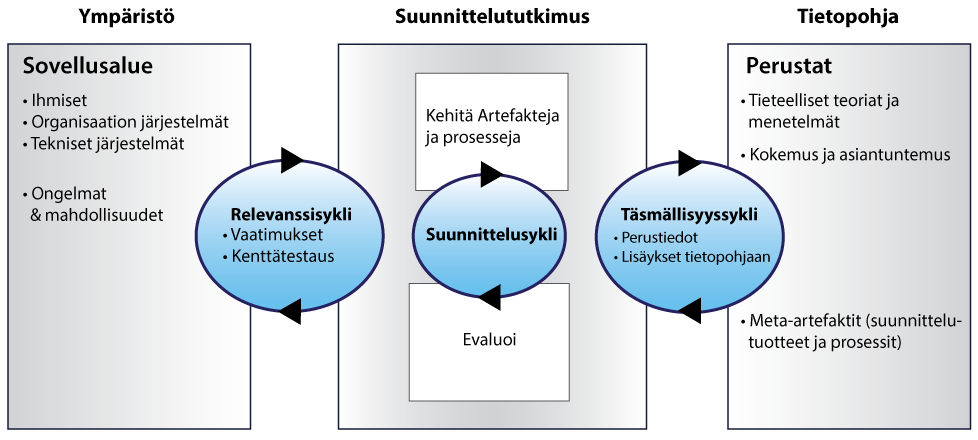
\includegraphics[height=7cm,keepaspectratio]{DSR}
  \caption{Suunnittelututkimuksen syklit Hevnerin \parencite*{cycles} laatimaa kuviota mukaillen. }
  \label{fig:dsr}
\end{figure}

Relevanssisykli on suunnittelututkimuksen aloittava sykli, joka määrittää vaatimukset ja evaluointikriteerit tutkimukselle sovellusalueella havaittujen ongelmien ja mahdollisuuksien pohjalta \parencite{cycles}. Hevner \parencite*{cycles} määrittelee sovellusalueen koostuuvan ihmisistä, organisaatiojärjestelmistä ja teknisistä järjestelmistä, jotka vuorovaikuttavat toistensa kanssa tietyn tavoitteen saavuttamiseksi. On kuitenkin otettava huomioon, että kaikkia ongelmia ja mahdollisuuksia ei välttämättä pystytä havaitsemaan etukäteen, sillä suunnittelutkimuksessa iteratiivisesti kehitettävä artefakti saattaa innovatiivisen luonteensa ansiosta tarjota ratkaisuja aivan uudenlaisiin ongelmiin \parencite{pragmatic}. Artefaktia koskevien evaluointitulosten peilaaminen ympäristöön on oleellinen osa relevanssisykliä, ja sen perusteella päätetään, vaatiiko tutkimus uusia relevanssi-iteraatioita \parencite{cycles}. 

Suunnittelututkimuksessa toteutettavan artefaktin kehitys ja evaluointi on suoritettava täsmällisin menetelmin, jotta tutkimustulokset olisivat valideja myös muussakin kuin tutkimuksen kontekstissa \parencite*{hevner2004}. täsmällisyyssyklin tarkoituksena on haalia tutkimukselle kattava tietopohja, johon sisältyvät tieteelliset teoriat, tekniset menetelmät, sovellusalueen kokemus ja asiantuntijuus sekä jo olemassa olevien artefaktien sen hetkinen tila \parencite{cycles}. Hevnerin \parencite*{cycles} mukaan tietopohjan perusteella saadaan myös selvyys siihen, onko kehitetty artefakti todella innovatiivinen. Hän myös toteaa, että tutkimuksessa luodut artefaktit, kokemukset, sekä laajennokset alkuperäisiin teorioihin ja menetelmiin ovat kontribuutioita tietopohjaa koskien. Iivarin mukaan \parencite*{pragmatic} täsmällisyys on se ominaisuus, mikä erottaa suunnittelututkimuksen tavallisesta artefaktien kehittämisestä.  On kuitenkin epärealistista olettaa, että aivan kaiken suunnittelutyön tulisi pohjautua ilmiöitä kuvaaviin teorioihin \parencite{cycles, pragmatic}. Iivari \parencite*{pragmatic} sen sijaan korostaa suunnittelututkimuksen läpinäkyvyyden merkittävyyttä, ja esittää artikkelissaan neljä sen toteutumista tukevaa ideoiden lähdettä:

\begin{enumerate}
  \item Käytännön ongelmat ja mahdollisuudet
  \item Jo olemassa olevat artefaktit
  \item Analogiat ja metaforat
  \item Teoriat
\end{enumerate}

Suunnittelututkimuksen tärkein sykli on suunnittelusykli, joka pitää sisällään artefaktin suunnittelun ja evaluoinnin \parencite{cycles}. Hevner \parencite*{cycles} tarkentaa, että syklin tarkoituksena on luoda erilaisia suunnittelutyön tuotoksia, arvioida niitä, ja tarkistaa vastaavatko ne relevanssisyklissä määritettyjä vaatimuksia. On myös oleellista, että artefaktien suunnittelu ja evaluointi toteutetaan täsmällisyyssyklissä määritettyjä teorioita ja mentelmiä hyödyntäen. Suunnittelusyklissä tapahtuu suurin osa suunnittelututkimuksen työstä, ja tästä syystä iteraatioita on tiheämmin kuin relevanssisyklissä tai täsmällisyyssyklissä, jotka luovat pohjan suunnittelusyklissä toteutettaville toimenpiteille \parencite{cycles}.

\subsection{Artefaktin evaluointi}
\label{kriteerit}

Artefaktin evaluointi on suunnittelututkimuksessa merkittävä toimenpide, jossa arvioidaan tietyin menetelmin, suoriutuuko artefakti sille määrätyistä tehtävistä tiettyjen kriteerien pohjalta \parencite{smith}. Suunnittelututkimuksen alkuvaiheilla on tärkeä määrittää mihin objektiin evaluointi kohdistuu, mitkä ovat evaluoinnin kriteerit, sekä määrittää kuinka artefaktin evaluointi suoritetaan ja mitä menetelmiä siinä käytetään \parencite{evaluation}. Se, että kehitetty artefakti on relevantti ja täsmällisesti toteutettu, ei riitä tekemään suunnittelututkimuksesta arvokasta, jos evaluointi on puutteellinen \parencite{cycles}. Ilman evaluointia suunnittelututkimuksen tuotokset ovat perustelemattomia suunnitteluteorioita tai hypoteesejä artefaktin ongelmanratkaisua koskien \parencite{comprehensive}. 

Vaikka evaluoinnin merkitystä korostetaankin kirjallisuudessa, tarkkaa tietoa sen suorittamisesta löytyy suhteellisen vähän, ja se on hajaantunut ympäriinsä \parencite{pries, comprehensive, evaluation}. On siis syytä käydä läpi erilaisia määritelmiä evaluoinnin strategioihin, menetelmiin ja kriteereihin liittyen. Ensinnäkin on olennaista tietää, minkä tyyppiseen artefaktiin evaluointi kohdistuu. Walls ym. \parencite*{walls} jaottelevat artefaktit prosessi- ja tuoteartefakteiksi, ja tätä kyseistä jaottelua on hyödynnetty kirjallisuudessa laajasti. Toinen oleellinen evaluointiin liittyvä kysymys koskee sen suoritushetkeä. Evaluointi voi olla tyypiltään ex-ante, jolloin evaluoidaan toteuttamatonta artefaktia, tai ex-post, jolloin evaluointi kohdistuu instanssoituun artefaktiin \parencite{pries}. Kolmas kysymys koskee evaluoinnissa hyödynnettäviä menetelmiä, jotka Venable \parencite*{venable} jaottelee joko keinotekoisiin tai naturalistisiin, eli todellisuutta vastaaviin menetelmiin. Edellä mainitut kolme evaluointiin liittyvää kysymystä perustuvat Pries-Hejen ym. \parencite*{pries} laatimaan viitekehykseen, jonka tarkoitus on tukea kirjallisuudessa esiintyvien evaluointien analysointia ja tarjota tutkijoille strategisia näkemyksiä evaluoinnin suorittamisesta. Kyseinen viitekehys on esitetty kuviossa \ref{fig:heje}.

\begin{figure}[H]\centering
  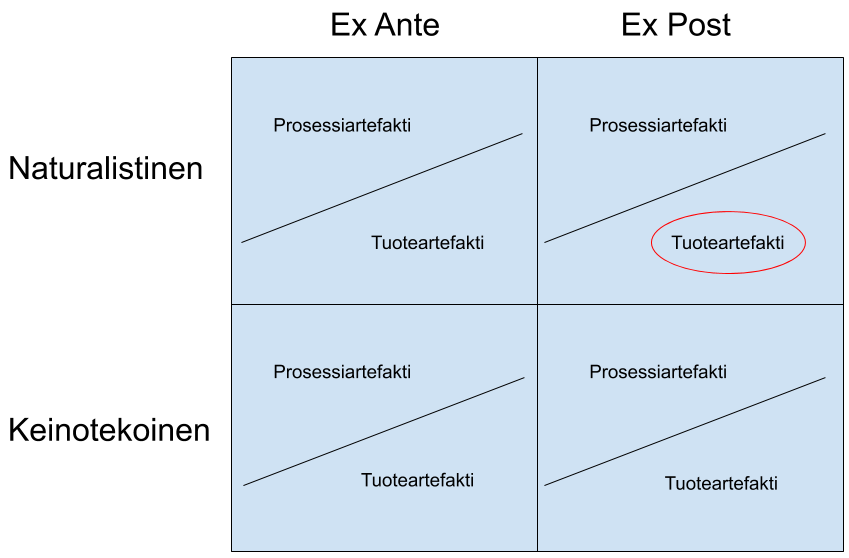
\includegraphics[height=8cm,keepaspectratio]{heje}
  \caption{Evaluoinnin ominaisuuksia kuvaava viitekehys Pries-Hejeä \parencite*{pries} mukaillen. Äänipalautetyökalun sijoittuminen viitekehykseen on merkattu punaisella rajauksella.}
  \label{fig:heje}
\end{figure}

Pries-Hejen ym. \parencite*{pries} laatima viitekehys ei kuitenkaan kerro, kuinka erilaiset evaluoinnin valintaan vaikuttavat tekijät tulisi ottaa huomioon strategiaa valittaessa \parencite{comprehensive}. Venable ym. \parencite*{comprehensive} ovat laajentaneet siitä oman kaksiosaisen viitekehyksen, mikä avustaa sekä evaluointistrategian että evaluointimenetelmän valinnassa. Se muistuttaa rakenteeltaan hyvin paljon alkuperäistä Pries-Hejen ym. \parencite*{pries} viitekehystä, mutta nelikkojen sisään on sijoitettu erilaisia vaatimuksia tai evaluointimenetelmiä, jotka avustavat valinnan tekemisessä. 

Venablen ym. \parencite{comprehensive} viitekehys taas ei esitä evaluointikriteereitä systemaattisesti, tai suhteuta niitä evaluointimenetelmiin, ja sama koskee muutakin kirjallisuutta \parencite{evaluation}. Prat, Comyn-Wattiau ja Akoka \parencite*{evaluation} ovat tästä syystä laatineet kirjallisuudessa hajallaan esiintyvistä evaluointikriteereistä hierarkian, jonka he ovat jakaneet systeemiteorian eri ulottuvuuksien mukaan. Tätä he perustelevat sillä, että Simonin \parencite*{simon1996}, ja monien muiden mukaan suunnitteluartefaktit voidaan mieltää järjestelmiksi. Hierarkian evaluointikriteerit on jaoteltu järjestelmän kanonisen muodon mukaisesti viiteen ulottuvuuteen, joihin kuuluvat: tavoite, ympäristö, rakenne, aktiivisuus ja evoluutio \parencite{modeling, systemic}. Prat ym. \parencite*{evaluation} ovat jakaneet nämä ulottuvuudet vielä useampiin alakriteereihin kirjallisuudessa esiintyvien evaluointikriteerien pohjalta. Hierarkia on esitetty kuviossa \ref{fig:evaluointikriteerit}, ja seuraavaksi tarkastellaan siinä esiintyviä evaluointikriteereitä.

Järjestelmän ulottuvuuksista tavoitteen alle on jaoteltu seuraavat evaluointikriteerit:  tehokkuus, validius sekä yleisyys. Tehokkuudella mitataan, kuinka hyvin artefakti onnistuu sille määrätyn tavoitteen saavuttamisessa, eli kuinka tarkoituksenmukainen se on. Validisuudella mitataan, saavuttaako artefakti sille määritetyt tavoitteet oikealla tavalla,  ja yleisyys vastaa artefaktin tavoitteen laajuudesta. \parencite{evaluation}

Hevnerin ym. \parencite*{hevner2004} mukaan artefaktin ympäristö koostuu ihmisistä, organisaatioista ja teknologiasta. Tämän pohjalta ympäristöä koskevan ulottuvuuden alle on sijoitettu seuraavat evaluointikriteerit: johdonmukaisuus ihmisten kanssa, johdonmukaisuus organisaation kanssa, sekä johdonmukaisuus uusimpien teknologioiden kanssa. Nämä evaluointikriteerit on vielä jaoteltu useampiin alakriteereihin, joista sekä ihmisten ja organisaation johdonmukaisuuden alle kuuluva hyödyllisyys mittaa, kuinka hyödyllinen artefakti on käytännössä. Ihmisten johdonmukaisuuteen liittyvät muut alakriteerit ovat ymmärrettävyys, helppokäyttöisyys, eettisyys sekä sivuvaikutukset. Organisaation johdonmukaisuutta koskevat alakriteerit ovat artefaktin yhteensopivuus organisaation kanssa ja artefaktin sivuvaikutukset. Teknologista johdonmukaisuutta koskevat alakriteerit ovat uusimpien teknologioiden valjastaminen ja sivuvaikutukset. \parencite{evaluation}

Järjestelmän rakenteeseen liittyvät evaluointikriteerit ovat artefaktin täydellisyys, yksinkertaisuus, selkeys, tyyli, homomorfismi, yksityiskohtaisuus ja johdonmukaisuus. Tämä järjestelmän ulottuvuus liittyy artefakteista malleihin, menetelmiin ja rakennelmiin, eikä siis koske instanssitasoisia artefakteja. \parencite{evaluation}

Järjestelmän ulottuvuuksista aktiivisuus liittyy artefaktin toimintaan, ja sitä koskevat evaluointikriteerit ovat: täydellisyys,  johdonmukaisuus, tarkkuus, suorituskyky sekä tehokkuus. Artefaktin toiminnan täydellisyys ja johdonmukaisuus liittyy sekä toiminnalliseen että rakenteelliseen näkökulmaan, ja tarkkuus varmistaa, että tulokset ovat linjassa muiden tutkimustulosten kanssa. Suorituskyky liittyy toiminnan nopeuteen tai suoritustehoon, sekä tehokkuus mittaa toiminnan syötteiden ja ulostulon välistä suhdetta. \parencite{evaluation}

Järjestelmän evoluutioon liittyvät evaluointikriteerit ovat vakaus (engl. robustness) ja oppimiskyky. Vakaudella tarkoitetaan artefaktin kykyä sopeutua ympäristön muutoksiin, ja oppimiskyvyllä sen kykyä oppia asioita aiemmista kokemuksista sekä ympäristön reaktioista. \parencite{evaluation}

Prat, Comyn-Wattiau ja Akoka \parencite*{evaluation} ovat laatineet evaluointikriteerien hierarkian lisäksi geneerisen mallin, jolla voidaan helpottaa evaluoinnin suunnittelua ja kuvata sen erilaisia ominaisuuksia. He jakavat evaluointimenetelmän viiteen eri komponenttiin, joita ovat evaluointikriteerit, evaluoinnin tyyppi, evaluoinnin taso, evaluoinnin suhteellisuus sekä toissijaiset osallistujat. Evaluoinnin tyyppi jaotellaan joko määrälliseksi tai laadulliseksi, joista määrällinen tuottaa jonkin mitatun tai havaitun numeerisen arvon \parencite{evaluation}. Evaluointi voi olla joko abstrakti- tai instanssi-tasoista, riippuen evaluoitavan artefaktin tyypistä, ja se voidaan suorittaa keinotekoisesti tai autenttisesti. Tämä artefaktin ja evaluoinnin tyypin luokittelu pohjautuu Pries-Hejen ym. \parencite*{pries} viitekehykseen. Evaluointi voi olla suhteellisuudeltaan absoluuttista, eli tarkoituksena on mitata työkalun suoriutumista itsessään, tai se voidaan suhteuttaa samankaltaisiin artefakteihin. Jos vastaavanlaista artefaktia ei ole vielä kehitetty, evaluointi on suhteessa samankaltaisten artefaktin puuttumiseen. Malli ottaa huomioon myös sen, hyödynnetäänkö evaluoinnissa toissijaisia osallistujia, kuten esimerkiksi oppilaita \parencite{evaluation}. Edellä mainituista evaluoinnin ominaisuuksista osa jakautuu vielä alaluokkiin.

\begin{figure}[H]\centering
\newgeometry{top=0cm}
  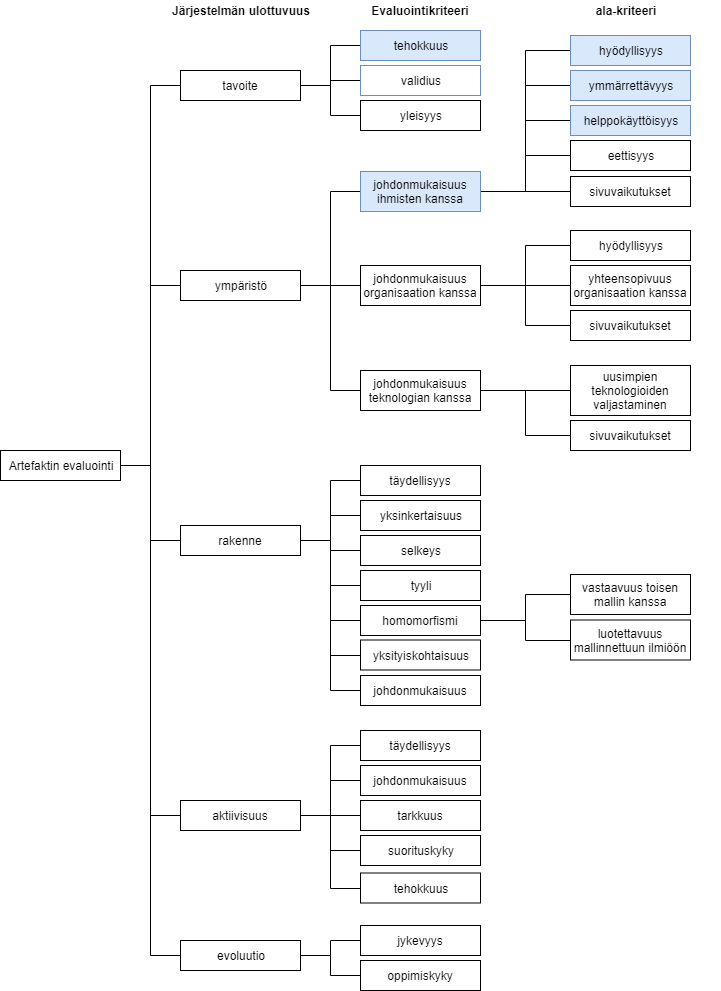
\includegraphics[width=\textwidth,height=\textheight,keepaspectratio]{evaluointikriteerit}
  \caption[]{Evaluointikriteerien hierarkia Pratin, Comyn-Wattiaun ja Akokan \parencite{evaluation} laatimaa kuviota mukaillen. Äänipalautetyökalun evaluointikriteerit on korostettu sinisellä värillä.}
  \label{fig:evaluointikriteerit}
\restoregeometry
\end{figure}

\section{Design science sovellettuna tähän tutkimukseen}

Tämä pro gradu -tutkielma pohjautuu suunnittelututkimukseen, jonka ominaisuuksia ja toteutusta käsiteltiin tarkemmin edellisessä luvussa \ref{design}. Tutkimuksen tavoitteena on suunnitella ja kehittää äänipalautteen antamiseen tarkoitettu työkalu, jonka avulla palautteenanto olisi mahdollisimman helppoa. Useiden tutkimusten mukaan äänipalautteen nauhoittamiseen ja jakamiseen liittyy erilaisia haasteita, joiden ylittäminen vaatii opettajilta teknistä osaamista. Tämä lähtökohta toimii pohjana työkalun suunnittelulle, jotta myös opettajat, joiden tietotekniset taidot eivät ole kovin korkeat, pystyisivät antamaan äänipalautetta sen avulla. Ratkaistava ongelma on siis äänipalautteen antamiseen liittyvä haasteellisuus, jota pyritään ratkomaan instanssitasoisella suunnitteluartefaktilla. Artefaktin evaluoinneilla pyritään vastaamaan seuraaviin ongelmista ja tavoitteista johdettuihin tutkimuskysymyksiin:

\begin{itemize}
  \item Helpottaako äänipalautetyökalu äänipalautteen antamista?
  \item Muuttaako äänipalautetyökalun käyttö suhtautumista äänipalautteen antamiseen?
\end{itemize}

Suunnittelututkimuksessa käsiteltävät ongelmat luokitellaan "viheliäisiksi ongelmiksi", joiden ratkaiseminen vaatii innovatiivisuutta (ks. luku \ref{design}). Äänipalautteen antamiseen liittyvien haasteiden minimointi voidaan luokitella tällaiseksi ongelmaksi useista eri syistä. Työkalun vaatimukset ja rajoitteet ovat projektin alussa epäselvät, sillä tarkoituksena on nimenomaan selvittää erilaisia artefaktia koskevia ratkaisuja, jotka helottavat äänipalautteen antamista. Tämä epätietietoisuus vaikuttaa myös siihen, että artefaktin suunnittelu ja toteutus muovaantuu prosessin edetessä, ja ongelmanratkaisu vaatii jatkuvasti luovaa ajattelua. Lisäksi tutkielman ohjaajien ja muiden työkalun evaluointiin osallistuvien henkilöiden kokemuksilla, näkemyksillä ja tulkinnoilla on suuri vaikutus artefaktin suunnittelu- ja toteutus-ratkaisuihin, sillä he kuuluvat työkalua hyödyntävään kohderyhmään, toisin kuin itse työkalun toteuttaja.

Suunnittelututkimuksen tavoitteena on yleensä organisaation toiminnan tehostaminen, mutta se ei ole tämän tutkielman tavoitteena. Sen sijaan prototyyppityökalun suunnittelulla ja toteutuksella pyritään kartoittamaan erilaisia äänipalauteen antamista helpottavia innovaatioita ja tuomaan ne ihmisten tietoisuuteen, jotta vastaavanlaisen työkalun toteuttaminen olisi helpompaa tulevaisuudessa. Tämä taas mahdollistaisi sen, että yhä useampi opettajista voisi hyödyntää äänipalautetta opetuksessaan.

\subsection{Tutkimuksen eri vaiheet}

Suunnittelututkimuksen toteutus voidaan jakaa kolmeen sykliin, joita suoritetaan iteratiivisesti sen elinkaaren lävitse tiettyyn pisteeseen saakka \parencite{cycles}. Niitä ovat relevanssisykli, täsmällisyyssykli, ja suunnittelusykli, joiden ominaisuuksia on käsitelty tarkemmin luvussa \ref{cycless}.  Jotta tutkimus vastaisi laajuudeltaan suurinpiirtein pro gradu -tutkielman laajutta, suunnittelututkimus joudutaan rajaamaan kahteen iteraatioon.

Tämä tutkimus alkaa relevanssisyklillä, jonka kautta saadaan alustavia vaatimuksia tutkimuksen toteutukselle ja äänipalautetyökalulle. Se kohdistuu tutkimuksen sovellusalueeseen, joka koostuu yliopistosta organisaationa, sen opetushenkilökunnasta sekä, äänipalautteen antamisessa hyödynnettävistä järjestelmistä. Ensisijaisena tavoitteena on selvittää miten opettajat suhtautuvat äänipalautteen antamiseen, mitä työkaluja he käyttävät siihen, millaisia haasteita he ovat prosessissa kohdanneet, sekä millä keinoin sitä voitaisiin mahdollisesti helpottaa. Alkuvaiheessa on myös oleellista määrittää artefaktin evaluointikriteerit, jotta työkalun kehityksessä osataan panostaa oikeisiin asioihin.

Relevanssisyklin kanssa samanaikaisesti suoritetaan myös täsmällisyyssykliä, jonka kautta kartoitetaan artefaktin kehitystä tukevaa tietopohjaa. Se aloitetaan tutkimalla erilaisia äänipalautteen nauhoittamisessa ja jakamisessa hyödynnettäviä menetelmiä ja työkaluja, jotta saadaan selville, mitkä asiat tukevat äänipalautteen antamista, ja mitä asioita voidaan vielä parantaa. Syklissä pyritään myös löytämään käyttöliittymän suunnittelua ohjaavia käytettävyysperiaatteita, jotta työkalun käytettävyys ja helppokäyttöisyys olisi perusteltua myös teoriatasolla. 

Kun alustavat vaatimukset on määritelty ja riittävä tietopohja äänipalautteen antamisesta hankittu, voidaan keskittyä työkalun varsinaiseen toteutukseen. Äänipalautetyökalun suunnittelusykli eroaa perinteisestä suunnittelututkimuksesta siten, että siihen sisältyy säännöllisin väliajoin järjestettävät tapaamiset jomman kumman, tai molempien ohjaajien kanssa. He kuuluvat äänipalautetta hyödyntävään kohderyhmään, joten heidän kokemuksistaan ja näkemyksistään on apua erilaisten suunnitteluratkaisujen määrittelyssä. Toinen tutkielman ohjaajista keskittyy enemmän teknisiin seikkoihin, kun taas toinen yleisempiin asioihin työkalua ja tutkielmaa koskien. Tapaamisissa työkalulle määritellään tiettyjä vaatimuksia, jotka tulee toteuttaa seuraavaan ohjauskertaan mennessä. Tapaamisissa myös evaluoidaan pienimuotoisesti työkaluun tehtyjä muutoksia, jotta varmistutaan, että kehityksen suunta on oikea. Tällainen inkrementaalinen ja iteratiivinen kehitystapa omaa piirteitä ketterästä ohjelmistokehityksestä.

\begin{figure}[h]\centering
  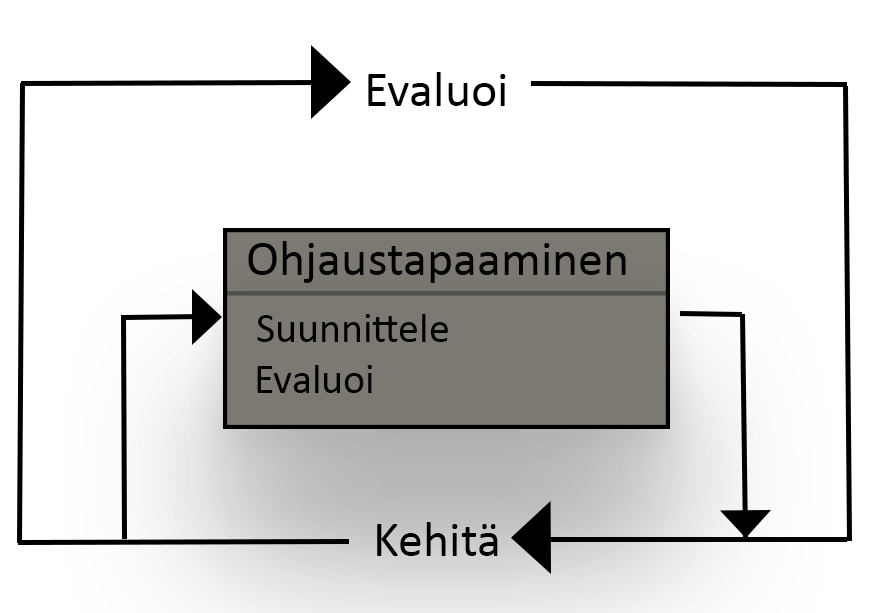
\includegraphics[height=10cm,keepaspectratio]{Kehitysvaihe}
  \caption{Äänipalautetyökalun kehitysprosessi.}
  \label{fig:kehitys}
\end{figure}

Kun prototyyppi on kehitetty siihen pisteeseen, että äänipalautteen antaminen onnistuu sen avulla, voidaan siirtyä ensimmäisen evaluoinnin pariin, joka on luonteeltaan formatiivinen. Siinä äänipalautetyökalua testataan ensimmäistä kertaa äänipalautteen antamisessa, joten on odotettavissa, että työkalusta löytyy puutteellisuuksia. Ensimmäisessä evaluoinnissa esille nousseiden tulosten pohjalta työkalua parannellaan siltä osin kun mahdollista, jonka jälkeen työkalu on valmis evaluoitavaksi toiseen kertaan. Se on tutkimuksen tärkein osuus, sillä siinä esille nousseiden tulosten pohjalta pyritään löytämään vastauksia tutkielman tutkimuskysymyksiin. Evaluointien suoritusta ja evaluointikriteereitä käsitellään yksityiskohtaisemmin seuraavassa luvussa \ref{eval}.

\subsection{Artefaktin evaluointi}
\label{eval}

Tässä tutkielmassa suoritetaan kaksi evaluointia, jotka kohdistuvat instanssitasoiseen artefaktiin, äänipalautetyökaluun. Evaluointien pohjalta on tarkoitus selvittää, helpottaako tetyökalu äänipalautteen antamista, tai muuttaako se suhtautumista sen antamiseen. Evaluointiin osallistuu neljä informaatioteknologian alan opettajaa, joista ainoastaan kaksi osallistuu ensimmäiseen evaluointiin. Testihenkilöt voivat suorittaa evaluoinnin joko mobiililaitteella, tabletilla tai tietokoneella, eikä evaluoinnin suoritus ole paikasta riippuvainen, sillä on tärkeää, että artefaktia testataan todellisessa ympäristössään \parencite{smith}.

Jokainen evaluoinnin suorittavista testihenkilöistä on hyödyntänyt äänipalautetta opetuksessaan, joten he pystyvät vertaamaan äänipalautetyökalua aiemmin käyttämiinsä audio-ohjelmistoihin. Tämän johdosta evaluoinnin suhteellisuuden voidaan määritellä olevan suhteessa samankaltaisiin ohjelmistoihin, mutta koska vastaavanlaista äänipalautetyökalua ei ole saatavilla, evaluointi on myös suhteessa vastaavanlaisten artefaktien puuttumiseen. Tavoitteena ei kuitenkaan ole ainoastaan artefaktin vertaaminen muihin audio-ohjelmistoihin, vaan mitata absoluuttisesti, kuinka hyvin äänipalautetyökalu tukee tarkoitustaan eli äänipalautteen antamista.

Evaluointikriteerit on tärkeä määritellä ennen evaluointia, ja niiden valintaan vaikuttavat erilaiset tavoitteet artefaktin suhteen. Äänipalautetyökalun tapauksessa ne on valittu Pratin, Comyn-Wattiaun ja Akokan \parencite*{cycles} laatimasta evaluointikriteerien hierarkiasta, joka on koottu kirjallisuudessa esiintyvien kriteerien pohjalta. Yhdeksi evaluointikriteeriksi valittiin tehokkuus, tarkemmin tarkoituksenmukaisuus, joka vastaa siitä, kuinka hyvin artefakti suoriutuu sille asetetusta tehtävästä, eli tässä tapauksessa äänipalautteen antamisesta. Toinen valituista evaluointikriteereistä on johdonmukaisuus ihmisten kanssa, joka jakautuu vielä viideksi alakriteeriksi. Näistä alakriteereistä valinta kohdistui hyödyllisyyteen, ymmärrettävyyteen ja helppokäyttöisyyteen. Ulkopuolelle rajattiin eettisyys ja sivuvaikutukset, sillä ne eivät ole tämän tutkimuksen kannalta oleellisia. Järjestelmän ulottuvuuksista rakenteeseen, aktiivisuuteen ja evoluutioon liittyvät kriteerit rajattiin suoraan ulos, sillä ne eivät ole oleellisia instanssoidun prototyypin kannalta. Evaluointikriteerien hierarkia on esitetty kuviossa \ref{fig:evaluointikriteerit}, jossa äänipalautetyökalun evaluointikriteerit on korostettu sinisellä värillä. Niiden toteutumista analysoidaan laadullisesti evaluoinnin tuloksien pohjalta.
 
Evaluoinnissa opettajien tulee käyttää työkalua äänipalautteen antamiseen autenttisessa tilanteessa. Tarkemmin sanottuna voidaan puhua simuloidusti autenttisesta tilanteesta, sillä opettajat eivät voi hyödyntää nauhoittamaansa äänipalautetta, koska palautteen tallentamismahdollisuutta ei ehditty toteuttamaan tämän tutkimuksen puitteissa. Kun testihenkilö on antanut äänipalautteen työkalun avulla, hänen tulee varmistaa, että hän on kokeillut jokaista työkalun perustoimintoa. Tämän jälkeen testihenkilö voi siirtyä evaluoinnin seuraavaan vaiheeseen, eli vastaamaan kyselylomakkeella esitettyihin kysymyksiin. Kysymykset ovat molemmissa evaluoinneissa samat, sillä poikkeuksella, että toiseen evaluointiin on lisätty osio navigointitoimintoja koskien, jotka lisättiin työkaluun ensimmäisen evaluoinnin tulosten pohjalta.

Kysely järjestetään puolistrukturoituna Google Forms verkkokyselynä, johon testihenkilöt saavat linkin sähköpostitse. Kyselylomake löytyy tutkielman liitteen \ref{lomake} osoittamasta linkistä. Lomakkeen alussa on esitetty evaluoinnin suoritusohjeet ja työkalua koskevat rajoitteet, jonka jälkeen varsinainen kysely alkaa. Testattuaan äänipalautetyökalua ohjeiden mukaisesti testihenkilöt vastaavat lomakkeella esitettyihin kysymyksiin, jotka liittyvät työkalun seuraaviin eri osa-alueisiin:

\begin{enumerate}
  \item Käyttökokemus
  \item Navigointitoiminnot
  \item Perustoiminnot
  \item Vapaamuotoinen palaute työkalua koskien
  \item Kehitysideat
\end{enumerate}

Ensimmäisessä osiossa testihenkilön tulee vastata kysymyksiin koskien työkalun käyttökokemusta. Siinä testihenkilöltä kysytään, palveliko työkalu käyttötarkoitustaan, helpottiko se äänipalautteen antamista entuudestaan, tai muuttiko sen käyttö suhtautumista äänipalautteen antamiseen. Osion ensimmäinen kysymys koskee tarkoituksenmukaisuutta, eli artefaktin oleellisinta evaluointikriteeriä sekä kaksi muuta kysymystä on johdettu suoraan tutkimuskysymyksistä. Siispä tämä tutkimustulosten kannalta kyselyn tärkein osio.

Toinen osio liittyy ensimmäisen evaluoinnin pohjalta toteutettuihin navigointitoimintoihin. Siinä testihenkilön tulee vastata, kokiko hän niiden toiminnallisuuden ja visuaalisuuden selkeäksi. Kolmannessa osiossa käyttäjän on mahdollista esittää huomioita työkalun perustoimintojen ymmärrettävyydestä ja visuaalisuudesta toiminto kerrallaan. 

Neljännessä osiossa käyttäjällä on mahdollisuus ilmaista vapaamuotoisia huomioita työkalua koskien. Osion kuvauksessa testihenkilöä kuitenkin ohjeistetaan peilaamaan asioita käytettävyyteen ja tarkoituksenmukaisuuteen, sillä ne ovat artefaktin kannalta oleellisia evaluontikriteereitä, joihin pyritään saamaan yksityiskohtaisia vastauksia.

Viimeiseen osioon testihenkilön on mahdollista kirjata sellaisia kehitysideoita, jotka hänen mielestään tukevat tai helpottavat äänipalautteen antamista työkalun avulla. Hänen on myös mahdollista ottaa kantaa työkalusta ulosrajattuun perustoimintoon, joka mahdollistaa tekstikenttien lisäämisen äänipalautteen eri kohtiin.

\begin{table}[H]
\begin{adjustwidth}{-1.5cm}{}
\caption{Yhteenveto evaluoinnin ominaisuuksista}
\begin{tabular}{|l|l|l|l|l|}
\hline
\textbf{Kuvaus} & \textbf{evaluointikriteerit}                                                                                                                                                                             & \begin{tabular}[t]{@{}l@{}}\textbf{evaluoinnin} \\  \textbf{tyyppi}\end{tabular} & \begin{tabular}[t]{@{}l@{}}\textbf{evaluoinnin}\\ \textbf{taso}\end{tabular} & \begin{tabular}[t]{@{}l@{}}\textbf{evaluoinnin} \\ \textbf{suhteellisuus}\end{tabular}                                                                                  \\ \hline
\begin{tabular}[t]{@{}l@{}}Äänipalautetyökalun\\ tarkoituksenmukaisuuden, \\ käytettävyyden ja \\ hyödyllisyyden evaluointi.\end{tabular} & \begin{tabular}[t]{@{}l@{}}Tehokkuus \\ Hyödyllisyys\\ Ymmärrettävyys \\ Helppokäyttöisyys\end{tabular} & Laadullinen                                                   & Instanssi                                                  & \begin{tabular}[t]{@{}l@{}}Absoluuttinen, \\ suhteessa samankal-\\ taisiin artefakteihin,\\ ja suhteessa saman- \\ kaltaisten artefaktien \\ puuttumiseen.\end{tabular} \\ \hline
\end{tabular}
\end{adjustwidth}
\end{table}

\chapter{Työkalun suunnittelu ja toteutus}

Tässä luvussa käsitellään äänipalautetyökalu prototyypin suunnittelu- ja toteutusratkaisuja eri näkökulmista. Aluksi läpikäydään työkalun tekniseen toteutukseen liittyviä seikkoja, jonka jälkeen käsitellään käyttöliittymän suunnittelua ohjaavia käytettävyysperiaatteita sekä itse käyttöliittymää. Lopuksi esitetään työkalun perus- ja erikoistoiminnot, sekä perustellaan valintoja niiihin liittyen. Linkki äänipalautetyökaluun löytyy litteestä \ref{tool}.

\section{Tekniset toteutusratkaisut}

Äänipalautetyökalun yksi tärkeimmistä vaatimuksista on se, että sitä voidaan käyttää vaivattomasti laitteella kuin laitteella ilman erillistä asennusta. Tämän vuoksi työkalu toteutetaan web-pohjaisena sovelluksena, eli sitä pystytään käyttämään selaimen välityksellä tietyn www-osoitteen kautta. Jotta tämä onnistuu, sovelluksen täytyy sijaita jollain palvelimella. Ensimmäisen iteraation ajan työkalu oli sijoitettuna Google App Engine -palveluun, mutta kokeilujakson päätyttyä se siirrettiin Heroku-palveluun, joka tarjoaa web-sovellusten verkkoisännöintiä täysin maksutta. 

Työkalu toteutettiin yhdestä näkymästä koostuvana staattisena verkkosivuna, sillä siten protoyyppi valmistuu nopeiten. Web-pohjaisuuden takia sovelluksen toteutustekniikat ovat selkeitä: rakenteen toteutuksessa käytetään HTML-merkintäkieltä, elementtien asettelussa CSS3-tyyliohjeita sekä toiminnallisuuksien toteutuksessa JavaScript-ohjelmointikieltä. Javascript-kehityksessä hyödynnetään jQuery-kirjastoa helpottamaan tiettyjä toimenpiteitä, kuten DOM-elementtien manipulointia. JQueryn lisäksi kehityksessä ei hyödynnetä muita kirjastoja tai ohjelmistokehyksiä, sillä ylimääräisiltä riippuvuuksilta halutaan välttyä jatkokehitystä ajatellen. Lisäksi tämä on hyvä mahdollisuus oppia Javascript ohjelmointikieltä sellaisenaan kuin se on. Ääniaallon piirtämiseen harkittiin wavesurfer-kirjastoa, mutta sen integrointi äänipalautetyökaluun olisi vaatinut enemmän aikaa kuin sen toteuttaminen itse verkosta haettujen ohjeiden avulla.

Työkalun nauhoitus on toteutettu MediaRecorder web-ohjelmointirajapintaa hyödyntäen. Se mahdollistaa äänen ja videon kaappaamisen tietovirtana selaimen kautta. Tutkimuksen toteutushetkellä selainten tuki kyseiselle ohjelmointirajapinnalle ei ole täysin kattava, sillä Safari-selaimen eri versiot tukevat sitä ainoastaan osittain. Nauhoittaminen voitaisiin tehdä myös vaihtoehtoisella tavalla, mikä mahdollistaisi nauhoittamisen myös Safarilla, mutta tämän prototyypin kannalta parhaaksi vaihtoehdoksi nähtiin MediaRecorder rajapinta.

\section{Hyödynnetyt käytettävyysperiaatteet}
\label{Kaytettavyysperiaatteet}


Äänipalautetyökalun suunnittelussa ja käytettävyyden arvioinnissa hyödynnetään erilaisia heuristiikkoja, jotta työkalun käytettävyys olisi mahdollisimman hyvä. Hyödynnettäviä käytettävyysperiaatteita ovat Gestaltin hahmolait, jotka käsittelevät erilaisten kuvioiden ja kokonaisuuksien visuaalista hahmottamista, sekä käytettävyysasiantuntija Jakob Nielsenin laatimat käytettävyysheuristiikat, jotka ovat vakiinnuttaneet asemansa ohjelmistokehityksen saralla jo 90-luvulta saakka.

Käytettävyydellä on suuri merkitys ohjelmistojen suunnittelussa ja arvioinnissa. Nielsenin mukaan \parencite*{intro-usability} käytettävyys on laatuattribuutti, jolla mittataan käyttöliittymän helppokäyttöisyyttä. Hän toteaa, että sillä viitataan myös kehitysprosessin aikaisiin toimiin, joilla pyritään parantamaan käyttöliittymän helppokäyttöisyyttä.

Nielsenin \parencite*{intro-usability} mukaan käytettävyys voidaan määrittää viidellä eri laatukomponentilla: opittavuudella, tehokkuudella, muistettavuudella, virheiden tekemisellä ja niistä toipumisella sekä käyttömukavuudella. Opittavuudella tarkoitetaan sitä, kuinka helppo käyttäjän on ensimmäistä kertaa käyttöliittymän kohdattaessaan suorittaa erilaisia perustoimenpiteitä, ja tehokkuudella sitä, kuinka nopeasti nämä toimenpiteet suoritetaan. Muistettavuudella tarkoitetaan sitä, kuinka nopeasti käyttäjä pystyy uudelleensaavuttamaan käyttötehokkuuden tietyn pituisen tauon jälkeen. Virheiden tekeminen, ja niistä toipuminen kattaa käyttäjän tekemien virheiden kokonaismäärän, kuinka vakavia ne ovat, sekä kuinka helposti näistä virheistä voidaan toipua. Käyttömukavuudella tarkoitetaan sitä, kuinka miellyttäväksi käyttäjä kokee käyttöliittymän.

Edellämainittujen laatuattribuuttien lisäksi on myös monia muita tärkeitä laatuattribuutteja, joista yksi on hyödyllisyys. Sillä mitataan, kuinka hyvin käyttöliittymän avulla pystytään tekemään juuri se, mitä käyttäjä tarvitsee \parencite{intro-usability}. Se on äänipalautetyökalun käytettävyyden arvioinnissa tärkeässä roolissa, sillä työkalun käyttötarkoitus on hyvin tarkkarajainen. 

\subsection{Gestaltin hahmolait}

Gestaltin hahmolait ovat periaatteita, jotka selittävät, kuinka ihmisaivot ryhmittelevät yksittäisiä visuaalisia elementtejä näkemästään ympäristöstä \parencite{koffka}. Hahmolait perustuvat 1800-luvulla alkunsa saaneeseen Gestalt-psykologiaan, joka tutkii kokonaisuuden ymmärtämistä sen yksittäisten osiensa sijaan. Max Wertheimerin vuonna 1923 julkaisemassaan artikkelissa "Untersuchungen zur Lehre von der Gestalt. II", hän käsittele havaisemiseen liittyviä lakeja ja niiden perusongelmia. Sillä oli Gubermanin ja Shelian \parencite*{rearranged} mukaan merkittävä vaikutus Gestalt-psykologiaan ja myös muihin tieteenaloihin, joten sitä voidaan pitää hahmolakeihin liittyvän kirjallisuuden yhtenä merkittävimpänä julkaisuna. 

Ajan saatossa Gestaltin hahmolaeista on ilmestynyt lukuisia eri variaatioita, mutta ne ovat usein keskenään samankaltaisia ja sisältävät päällekäisyyksiä. Gestalt-psykologiaa voidaan soveltaa useisiin eri tarkoituksiin, joten hahmolaeista joudutaan usein valitsemaan sopivimmat vaihtoehdot tapauskohtaisesti. Chang ym. \parencite*{chang} ovat koonneet tutkimukseensa 11 hahmolakia, joita he hyödyntävät opetuskäyttöön tarkoitetun ohjelmiston visualisessa suunnittelussa. Tässä tutkimuksessa hyödynnetään kyseistä hahmolakien joukkoa, ja se on esitetty seuraavassa listauksessa:

\begin{enumerate}
  \item Symmetrian laki
  \item Jatkuvuuden laki
  \item Sulkeutuvuuden laki
  \item Kohteen ja alustan laki
  \item Keskipisteen laki
  \item Yhdenmukaisuuden laki
  \item Hyvän muodon laki
  \item Läheisyyden laki
  \item Samankaltaisuuden laki
  \item Yksinkertaisuuden laki
  \item Yhtenäisyyden laki
\end{enumerate}

Symmetrian lain mukaan symmetrinen kuvio havainnoidaan kokonaisuudeksi sitä vahvemmin, mitä symmetrisempi kuvio on. Jatkuvuuden lain mukaan taas viivat, jotka jatkavat risteyskohdasta mahdollisimman samaan suuntaan, tulkitaan samaksi viivaksi. Sulkeutuvuuden lain mukaan tietty kuvio tulkitaan kokonaisuudeksi, vaikka siinä olisi puutteellisia osia. Kohteen ja alustan lain mukaan kohde, ja sen alusta tulkitaan eri tavalla niissä käytetyistä väreistä riippuen. Keskipisteen lain mukaan jokin muista erottuva kokonaisuus kiinnittää käyttäjän huomion ensin. Yhdenmukaisuuden lain mukaan kuvioiden tulkintaan vaikuttavat aiemmat siihen liittyvät kokemukset. 

Äänipalautetyökalun käyttöliittymä on yksinäkymäinen staattinen verkkosivu, joka koostuu  äänileikenäkymästä sekä perustoimintojen ja erikoistoimintojen painikkeista. Koska käyttöliittymän on tarkoitus olla mahdollisimman yksinkertainen, kaikkia edellä mainittuja heuristiikkoja ei välttämättä hyödynnetä käyttöliittymän suunnittelussa. Siitä huolimatta listauksesta voi olla apua jatkokehitystä ajatellen. 

\subsection{Nielsenin heuristiikat}

Jakob Nielsen on yksi maailman tunnetuimmista käytettävyysasijantuntijoista. Hän on työskennellyt käytettävyyyden parissa 90-luvulta saakka. Nielsen ja Molich \parencite*{improving-human} ovat määritelleet yhdeksän erilaista käytettävyysheuristiikkaa järjestelmän käytettävyyden arviointiin. Nielsen \parencite*{enhancing} jalosti myöhemmin näiden heuristiikkojen pohjalta päivitetyn listauksen, joka on validi ja laajasti käytetty yhä lähes kaksikymmentä vuotta myöhemmin. Heuristiikat on esitetty taulukossa \ref{nielsen}.

Käyttöliittymän käytettävyyden arviointi toteutetaan useimmiten heuristisesti, eli käyttöliittymää tarkastellaan ja siitä pyritään löytämään toimivat ja ei-toimivat ominaisuudet. Se on halpa ja intuitiivinen tapa havaita käyttöliittymän käytettävyysongelmat, eikä se vaadi erityistä etukäteissuunnittelua. Lisäksi sitä voidaan hyödyntää jo suunnitteluprosessin varhaisessa aiheessa, ja ihmisten motivointi sen suorittamiseen on helppoa. \parencite{heuristic-evaluation}

Heuristinen arviointi voidaan suorittaa oman intuition tai "maalaisjärjen" pohjalta, mutta Nielsen ja Molich \parencite*{heuristic-evaluation} ovat laatineet tarkoitusta varten omat heuristiikkansa, jotka kattavat yleisimmät käytettävyyteen liittyvät ongelmat. Nielsenin heuristiikkojen lisäksi on olemassa myös monia muita käytettävyysheuristiikkoja, joista parhaan valitseminen on yhä avoin kysymys \parencite{enhancing}. 

Heuristisessa evaluoinnissa ei tulisi luottaa ainoastaan yhden ihmisen arviointiin, vaan arvioijia olisi hyvä olla kolmesta viiteen \parencite{heuristic-evaluation}. Tässä tutkimuksessa heuristiikkojen toteutumista ei kuitenkaan arvioida erillisillä evaluoinneilla, vaan niitä hyödynnetään käyttöliittymän suunnittelussa Gestaltin hahmolakien rinnalla.

% Table generated by Excel2LaTeX from sheet 'Sheet1'
\begin{table}[H]
  \centering
  \caption{Nielsenin \parencite{heuristics} heuristiikat}
    \begin{tabular}{p{12.355em}p{21.855em}}
    \multicolumn{1}{l}{\textbf{Järjestelmän tilan näkyvyys}} & Järjestelmän tulisi informoida käyttäjälle tapahtumista asianmukaisilla palautteilla riittävän nopeasti. \\
    \textbf{Järjestelmän ja reaalimaailman yhtenäisyys} & Järjestelmän kielellisen sisällön tulisi olla käyttäjän ymmerrättävissä. Tiedon tulisi myös näyttäytyä luonnollisessa ja loogisessa järjestyksessä. \\
    \multicolumn{1}{l}{\textbf{Käyttäjän hallinta ja vapaus}} & Käyttäjät tekevät usein virheitä, joten ei-toivotusta tilasta tulisi päästä pois helposti esim. peruuta- ja palauta -toiminnoilla. \\
    \multicolumn{1}{l}{\textbf{Yhdenmukaisuus ja standardit}} & Erilaisten sanojen, tilanteiden ja toimintojen tulisi olla yhdenmukaisia, ja Järjestelmän tulisi myös noudattaa tunnettuja käytänteitä. \\
    \multicolumn{1}{l}{\textbf{Virheiden estäminen}} & Järjestelmän tulisi ensisijaisesti toimia siten, että virheitä ei pääsisi tapahtumaan. Virheelle alttiissa tilanteessa käyttäjältä tulisi pyytää varmistus toimenpiteen jatkamisesta. \\
    \textbf{Tunnistaminen muistamisen sijaan} & Käyttäjän muistamisen tarve tulisi minimoida pitämällä oleelliset objektit, toiminnot ja valinnat näkyvillä. Ohjeet järjestelmän käyttämiseen tulisi olla myös joko näkyvillä tai helposti saatavilla. \\
    \multicolumn{1}{l}{\textbf{Joustavuus ja käytön tehokkuus}} & Oikopolut erilaisille toimenpiteille nopeuttaa usein järjestelmän käyttöä, joten niiden tarjoaminen kokeneemmille käyttäjille on usein kannattavaa.  \\
    \textbf{Esteettisyys ja minimalistinen suunnittelu} & Tarpeetonta informaatiota dialogeissa tulisi välttää, sillä se vie näkyvyyttä relevantilta informaatiolta. \\
    \textbf{Virheiden tunnistaminen ja virheistä toipuminen} & Virheviestien tulisi olla selkokielisiä, sekä niiden tulisi täsmällisesti osoittaa millainen virhe on kyseessä ja miten siitä pystytään toipumaan. \\
    \textbf{Avustus ja dokumentaatio} & Dokumentaation tarjoaminen on useimmiten tarpeen, ja käyttäjän tulisi pystyä löytämään sieltä kaikki tarvittava informaatio pystyäkseen käyttämään järjestelmää. \\
    \end{tabular}%
  \label{tab:addlabel}%
\end{table}%

\section{Käyttöliittymä}
\label{Kayttoliittyma}

Käyttöliittymä on järjestelmän osa, jonka kautta käyttäjä on vuorovaikutuksessa järjestelmän kanssa saavuttaakseen tietyn tavoitteensa \parencite{stone}. Äänipalautetyökalun tapauksessa käyttötarkoitus on hyvin rajattu, joten käyttöliittymän tulee tukea sitä tehokkaasti ja käyttäjäystävällisesti. Käyttöliittymissä on usein eroja erilaisten järjestelmien välillä, sillä vuorovaikutuksessa käytetään erilaista välineitä, jotka vaikuttavat käyttöliittymäsuunnitteluun \parencite{stone}. Äänipalautetyökalun yksi oleellisista vaatimuksista on se, että sitä on pystyttävä käyttämään tietokoneilla, tableteilla ja puhelimilla, joten käyttöliittymä oli suunniteltava siten, että sen käyttö onnistuu hiiren ja näppäimistön lisäksi myös kosketusnäytöllä. Lisäksi käyttöliittymän skaalautuvuus on otettava huomioon, sillä päätelaitteiden ruudun koko vaikuttaa merkittävästi siihen, kuinka käyttöliittymän komponentit asettuvat siihen. Käyttöliittymä on esitetty tietokone-koossa kuvassa \ref{fig:UI}, tabletti-koossa kuvassa \ref{fig:UI_tablet} ja mobiili-koossa kuvassa \ref{fig:UI_mobile}.

Käyttöliittymän suunnittelun apuna hyödynnetään usein erilaisia käytettävyysperiaatteita, joilla käyttöliittymän suunnitteluratkaisuja voidaan perustella. Äänipalautetyökalun käyttöliitymän suunnittelussa on hyödynnetty Nielsenin heuristiikkoja ja Gestaltin hahmolakeja, jotka on käsitelty tarkemmin luvussa \ref{Kaytettavyysperiaatteet}. Tässä luvussa esitellään äänipalautetyökalun käyttöliittymä kokonaisuudessaan, ja peilataan tehtyjä suunnittelu- ja toteutusratkaisuja hyödynnettyihin käytettävyysperiaatteisiin. Luvussa esitetty käyttöliittymä on suunnittelututkimuksen toisessa iteraatiossa evaluoitu konfiguraatio, joten se eroaa hieman ensimmäisen evaluoinnin aikaisesta käyttöliittymästä. 

Äänipalautetyökalun käyttöliittymä voidaan jakaa vaakasuunnassa neljään eri alueeseen, joista kukin eroaa selvästi toisistaan. Työkalun yläosassa sijaitsevat avustusikkunan avaava kysymysmerkki-ikoni, siniset erikoistoimintopainikkeet sekä peruuta- ja palaa-toiminnot. Keskiössä sijaitsee muusta taustasta selkeästi erottuva äänileikenäkymä, joka on aikajana, johon nauhoitetut äänileikkeet ääniaaltoineen piirretään ja asetetaan. Äänileikenäkymän alapuolella sijaitsevat pallomaiset navigaatiotoiminnot, jotka toteutettiin ensimmäisen iteraation evaluointitulosten pohjalta. Käyttöliittymän alareunassa sijaitsevat perustoiminnot, joiden avulla varsinainen äänipalautteen nauhoittaminen ja editointi suoritetaan. 

Edellä mainittujen osioiden sijoittelulla ja ulkoasulla on suuri merkitys työkalun käytettävyyteen. Niiden tulee erottua toisistaan erillisiksi, selkeiksi kokonaisuuksiksi, joilla on oma tehtävänsä. Käyttöliittymän komponenttien sijoittelu ja asettelu on tehty mahdollisimman symmetriseksi ja tasapainoiseksi kokonaisuudeksi, ilman että yhtäkään toiminnallisuutta olisi piilotettu käyttäjältä. Gestaltin symmetrian lain mukaan tasapainoinen, eli keskiviivan molemmin puoleinen asettelu koetaan selkeämmäksi kuin epäsymmetrinen asettelu. Nielsenin tunnistaminen muistamisen sijaan -heuristiikka koskee sitä, että käyttöliittymän toiminnallisuuksien tulisi olla esillä ja mahdollisimman helposti saatavilla. Tämä myös toteutuu käyttöliittymässä. Edellä mainittujen seikkojen lisäksi käyttöliittymä on suunniteltu visuaalisuudeltaan mahdollisimman selkeäksi kokonaisuudeksi, ja siinä ei ole lainkaan epäolennaista informaatiota. Se on siis linjassa myös Nielsenin esteettinen ja minimalistinen suunnittelu -heuristiikan kanssa. Informaation määrää on vähennetty myös tietoisesti siten, että osa perustoimintojen painikkeista toimii kuten kytkimet, eli tietty toiminto aloitetaan ja keskeytetään samasta painikkeesta. Tällaisen toiminnon aktivoiduttua, muut perustoiminnot muuttuvat haaleiksi, indikoimaan sitä, etteivät ne eivät sillä hetkellä ole käytettävissä. Lisäksi aktivoidun painikkeen teksti muutetaan toiminnosta riippuen joko "Pause":ksi tai "Stop":iksi.

Gestaltin läheisyyden lain mukaan vierekkäiset elementit tulkitaan yhteenkuuluviksi, ja tätä periaatetta on hyödynnetty käyttöliittymän painikkeiden ryhmittelyssä. Käyttöliittymän erikoistoiminnot, peruuta- ja palaa-komennot, navigointipainikkeet sekä perustoiminnot ovat toiminnallisuuksiltaan selkeästi toisistaan eroavia, joten ne on ryhmitelty eri tavoin äänileikenäkymän ympärille. Perustoiminto-painikkeet muodostavat oman ryhmänsä, mutta myös niiden sisäisessä jaottelussa on hyödynnetty läheisyyden lakia. Record-, ja Insert Record -toiminnot ovat selvästi nauhoitukseen liittyviä toimintoja, joten ne on oma pienempi ryhmänsä. Play- ja Preview-toiminnot taas ovat äänitteiden toistamiseen liittyviä toimintoja, joten ne ovat oma itsenäinen ryhmänsä. Split- ja Delete-toiminnot liittyvät äänileikkeiden katkomiseen ja poistamiseen, joten myös ne ovat vahvasti liitoksissa toisiinsa. Läheisyyden lain mukaisesti, nämä kolme perustoimintojen ryhmää on erotettu toisistaan suuremmilla väleillä kuin toistensa kanssa samankaltaiset perustoiminnot. 

Gestaltin läheisyyden lain lisäksi elemettejä voidaan ryhmitellä myös samanlaisuuden lakia hyödyntäen. Sen mukaan kohteet voidaan tulkita samanlaiseksi värin, koon tai muodon perusteella. Läheisyyden lain lisäksi erityisesti painikkeissa hyödynnetään värin avulla ryhmittelyä. Erikoistoiminnot ovat korostettu sinisellä värillä, kun taas perustoiminnot ja niihin vahvasti niittyvät peruuta- ja palaa -toiminnot, on värjätty harmaalla, eli neutraalimmalla värillä. Navigointipainikkeet taas ovat väriltään vaalean harmaita, jota käytetään myös äänileikenäkymän taustavärinä. Tähän valintaan päädyttiin siksi, että äänileikkeiden välillä navigointi tapahtuu nimenomaan äänileikenäkymässä. Muista painikkeista eroten navigointipainikkeet ovat suorakaiteen sijasta ympyrän muotoisia, jotta ne erottuisivat selkeästi niiden alapuolella sijaitsevista perustoiminnoista. Koska uloimpien ja sisempien navigointipainikkeiden toiminnallisuuksissa on eroja, niin kaksi sisimmäistä painiketta on kooltaan kahta ulompaa painiketta suurempia. Lisäksi ulommissa ja sisemmissä painikkeissa sijaitsevien nuolien tyyli on hieman erilainen, jotta ne erottuisivat toisistaan muutenkin, kuin kooltaan.

Kaikissa käyttöliittymän painikkeissa, erikoistoiminnot poislukien, on hyödynnetty ikoneja, jotta ne olisivat mahdollisimman helposti ymmärrettäviä. Nielsenin johdonmukaisuus ja standardit -heuristiikan sekä Gestaltin yhdenmukaisuuden lain mukaan, käyttöliittymän tulisi sisältää tuttuja kuvioita, joiden tulkintaa helpottavat aiemmat kokemukset. Lähes jokainen työkalussa hyödynnetyistä ikoneista noudattaa kyseisiä käytettävyyseperiaatteita, mutta koska Insert Record on uudenlainen toiminto, jota ei löydy muista audio-ohjelmistoista, ikoni täytyi suunnitella toimintoa varten itse. Nielsenin johdonmukaisuuksin ja standardeihin liittyvä heuristiikka koskee kuvioiden lisäksi myös tekstiä, joten painiketeksteissä on noudatettu audio-ohjelmiston standardeja, siltä osin kuin mahdollista. Poikkeuksellisia ovat Insert Record -, ja preview-toiminnot, joille nimi jouduttiin määrittelemään itse. Insert tarkoittaa muun muassa väliin laittamista, joten Insert Record on kuvaava nimitys toiminnolle, joka nauhoittaa jo olemassa olevan äänileikkeen väliin uuden äänileikkeen. Preview-toiminto sen sijaan on vaikeampi päätellä pelkän tekstin pohjalta, mutta toiminnolle ei löydetty parempaa vaihtoehtoa, joka oltaisiin voitu esittää maksimissaan kahdella sanalla. Nielsenin heuristiikkojen mukaan järjestelmän tulisi puhua käyttäjän ymmärtämää kieltä, mikä on myös huomioitu painiketeksteissä ja avustusikkunan toimintojen kuvauksissa.

Johdonmukaisuutta ja standardeja on pyritty noudattamaan myös äänileikenäkymässä, joka koostuu aikajanasta, kursorista, vierityspalkista ja alueesta, johon nauhoitetut äänileikkeet sijoitetaan. Kuten useimmissa audio-ohjelmistoissa, aikajana sijaitsee äänileikenäkymän yläreunassa, ja nauhoitetut äänileikkeet sijoittuvat sen alapuolelle. Nauhoituksen edetessä, äänileikkeeseen piirretään reaali-ajassa ääniaalto, aivan kuten useimmissa audio-ohjelmistoissa, jotta äänitteen dataa voidaan tulkita myös visuaalisesti. 
Kun aikajanaa tai äänileikettä klikataan, punaisella värillä korostettu äänileikekursori siirettään haluttuun kohtaan, ja alla oleva äänileike korostetaan tummemmalla taustavärillä osoittamaan sitä, että se on asetettu valinnan kohteeksi.

Nielsenin käyttäjän hallinta ja vapaus -heuristiikan mukaan käyttäjän tulisi pystyä palaamaan ei-toivotusta tilasta, helposti ja tilanteesta riippumatta. Tätä heuristiikkaa tukee se, että työkaluun on toteutettu peruuta- ja palauta-toiminnot. Nielsenin heuristiikkojen mukaan käyttöliittymän tulisi olla myös joustava ja tehokas, joten tietyille toiminnoille on määritetty käyttöä tehostavat pikanäppäimet. Peruuta- ja palauta-toimintojen tapauksessa on noudatettu yleistä "CTRL + Z" ja "CTRL + Y" näppäinyhdistelmää, ja Delete-toiminnossa delete-näppäintä. Play-toiminto aktivoidaan välilyönnistä, aivan kuten useimmissa muissa audio-ohjelmistoissa. Navigointi äänileikenäkymässä on mahdollistettu nuolinäppäinten avulla, ja ensimmäisen evaluoinnin pohjalta toteutettu äänileikkeiden välillä navigointi voidaan navigointipainikkeiden lisäksi suorittaa myös "SHIFT + NUOLI" näppäinkomennolla.

Nielsenin heuristiikkojen mukaan virheiden tapahtuminen tulisi ensisijaisesti estää, ja sellaisen sattuessa, virheestä tulisi esittää selkeä kuvaus ja ohjeet siitä toipumiseen. Koska evaluoitava äänipalautetyökalu on prototyyppi, virheitä saattaa kuitenkin käytön aikana  ilmaantua. Toisen iteraation evaluoinnin ensimmäisenä suorittanut henkilö huomasi käyttöliittymää vilkaistessaan, ennen ohjeistuksen lukemista, ettei erikoistoiminnoista tapahtunut mitään, ja informoi asiasta sähköpostitse. Tämän seurauksena erikoistoimintojen painikkeita muutettiin siten, että niitä painettaessa käyttäjälle ilmoitetaan niiden keskeneräisyydestä.

\begin{figure}[H]\centering
  \begin{adjustwidth}{-2.2cm}{}
  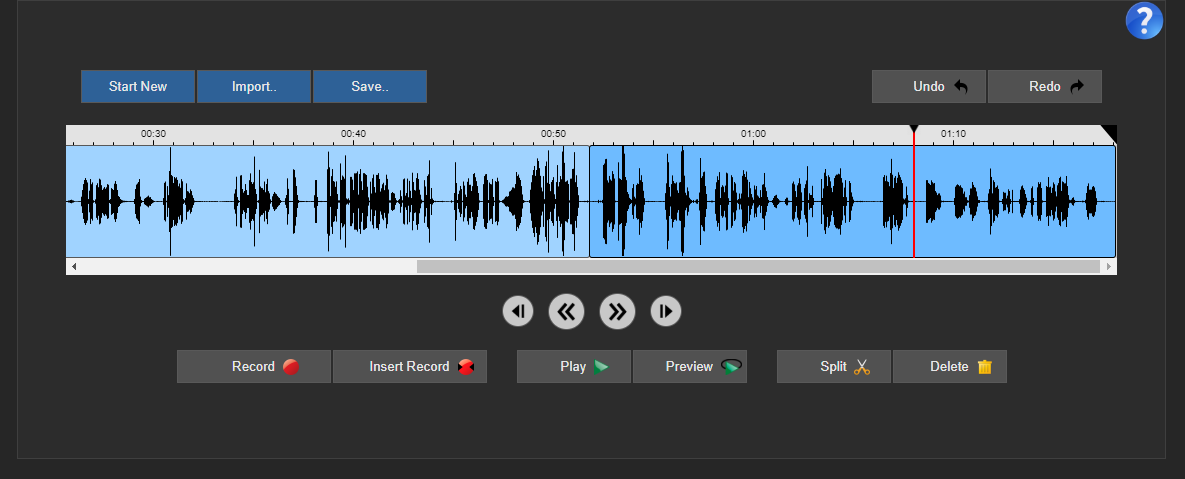
\includegraphics[height=7.5cm,keepaspectratio]{UI}
  \caption{Äänipalautetyökalun käyttöliittymä tietokone-koossa.}
  \label{fig:UI}
  \end{adjustwidth}
\end{figure}

\begin{figure}[H]\centering
  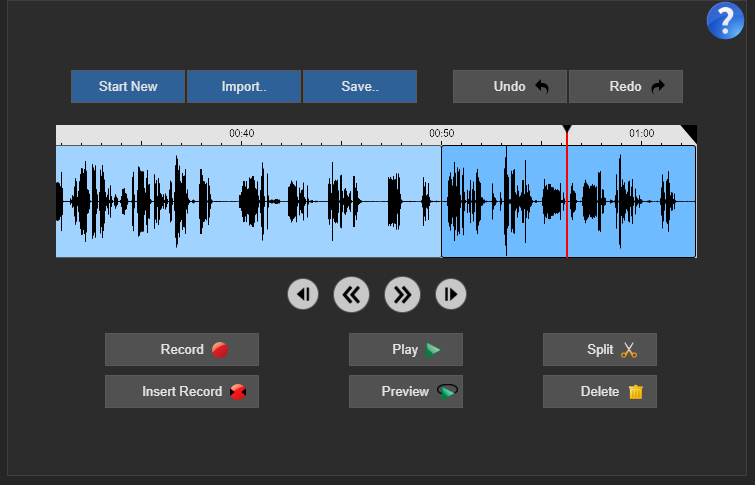
\includegraphics[height=8cm,keepaspectratio]{UI_tablet}
  \caption{Äänipalautetyökalun käyttöliittymä tabletti-koossa.}
  \label{fig:UI_tablet}
\end{figure}

\begin{figure}[H]\centering
  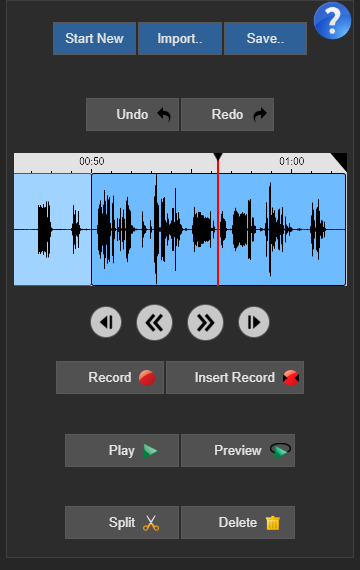
\includegraphics[height=9cm,keepaspectratio]{UI_mobile}
  \caption{Äänipalautetyökalun käyttöliittymä mobiili-koossa.}
  \label{fig:UI_mobile}
\end{figure}

\section{Perustoiminnot}

Äänipalautetyökalussa on kuusi perustoimintoa, joiden avulla äänitteiden nauhoittaminen, toistaminen ja editointi suoritetaan. Tässä luvussa käsitellään perustoimintojen ominaisuudet ja perustellaan miksi äänipalautetyökaluun on päätetty sisällyttää juuri kyseiset toiminnallisuudet. Perustoimintojen suunnittelu oli tutkielman yksi ensimmäisistä vaiheista, ja ne ovat pysyneet lähes samanlaisena koko kehityksen ajan. Toimintojen suunnitteluprosessi suoritettiin iteratiivisesti yhteistyössä ohjaajien kanssa, joiden kokemuksilla ja näkemyksillä oli vaikutusta lopputulokseen. Lisäksi päätöksiin vaikuttivat muiden audio-ohjelmistojen toiminnallisuudet, sillä standardien noudattaminen on useimmissa tapauksissa kannattavaa. Äänipalautetyökalu eroaa kuitenkin muista audio-ohjelmista siten, että äänileikkeitä ei ole mahdollista siirtää äänileikenäkymässä. Tähän on syynä se, että toiminnot on suunniteltu siten, ettei käyttäjän tarvitse siirtää äänileikkeiden paikkaa manuaalisesti, jotta työkalun käyttö olisi mahdollisimman intuitiivista ja tehokasta.

\subsection{Record}

Record-toiminto aloittaa äänipalautteen nauhoittamisen siihen kohtaan äänileikenäkymää, missä äänileikekursori sijaitsee nauhoituksen aloitushetkellä. Nauhoituksen tapahtuessa jo olemassa olevien äänileikkeiden päälle, uusi äänileike korvaa alle jääneet äänileikkeet. Nauhoitettava äänileike kasvaa nauhoituksen edetessä, ja äänileikekursoria liikutetaan äänileikkeen mukana. Kun äänileikekursori saavuttaa äänileikenäkymän oikean reunan, se pysäytetään, mutta nauhoitettava äänileike jatkaa levenemistään. Tällöin äänileikenäkymää vieritetään nauhoitettavan äänileikkeen mukaisesti, jolloin käyttäjä näkee ääniaallon piirtyvän äänikeikkeeseen reaaliajassa palautteenannon aikana. 

\subsection{Insert Record}

Insert Record -toiminto nauhoittaa uuden äänileikkeen jo olemassa olevan äänileikkeen väliin. Aluksi toiminto katkaisee äänileikkeen kahteen osaan, joiden väliin uusi äänileike nauhoitetaan. Tämän jälkeen uuden äänileikkeen nauhoittaminen aloitetaan, ja nauhoituksen edetessä, nauhoituskohdan oikealla puolella sijaitsevia äänileikkeitä liikutetaan nauhoitettavan äänileikkeen mukaisesti. Kuten tavallisessa nauhoituksessa, myös väliin-nauhoituksessa äänileikkeen ja kursorin saavuttaessa äänilekenäkymän oikean reunan, kursorin eteneminen pysäytetään, ja äänileikenäkymää aletaan vierittämään uuden äänileikkeen mukaisesti.

Jo perustoimintojen suunnitteluvaiheessa tuli ilmi, että äänipalautteen antamisessa on tarve uusien äänileikkeiden lisäämiselle palautteen väliin. Tämän pohjalta Insert Record toimintoa lähdettiin suunnittelemaan, ja tavoitteena oli tehdä siitä mahdollisimman helppo ja tehokas. Perinteisissä audio-ohjelmistoissa kyseinen toimenpide suoritettaisiin siten, että äänileike katkaistaisiin manuaalisesti halutusta kohdasta, nauhoitettaisiin uusi äänileike, ja aseteltaisiin pätkät oikeille paikoilleen. Insert Record -toiminto yhdistelee näitä kaikkia toimenpiteitä, ja se on osoittautunut erittäin toimivaksi.

\subsection{Play}

Play-toiminto aloittaa äänipalautteen toistamisen siitä kohdasta missä äänileikekursori sijaitsee toiston aloitushetkellä. Äänileikekursoria liikutetaan toiston edetessä eri tavoin riippuen sen sijainnista ja sitä ympäröivistä äänileikkeistä. Kursoria liikutetaan äänileikenäkymässä oikealle päin siihen asti, kunnes se melkein saavuttaa äänileikenäkymän oikean reunan. Kursorin ja äänileikenäkymän oikean reunan välille jätetään pieni väli, jotta toiston edetessä nähdään pieni tulossa oleva pätkä toistettavasta äänileikkeestä. Jos äänileikenäkymässä on vieritysvaraa oikealle päin, eli toisin sanoen kursoria seuraavia äänileikkeitä, niin äänileikekursori pysähtyy paikalleen ja äänileikenäkymää vieritetään oikealle päin. Kun äänileikenäkymä saavuttaa sen pisteen, ettei vieritettävää enää ole, niin se luonnollisesti pysähtyy ja äänileikekursoria liikutetaan oikealle, kunnes äänileikenäkymän oikea reuna saavutetaan.
 

\subsection{Preview}

Preview-toiminto toimii lähes samalla tavalla kuin Play-toiminto, eli aloittaa äänipalautteen toiston siitä kohdasta, missä äänileikekursori toiston aloitushetkellä sijaitsee. Ainut eroavaisuus tavalliseen toistamiseen on se, että toiston loputtua äänileikekursori palautetaan toiston aloituskohtaan. Tämä toiminto päätettiin sisällyttää toteutukseen, sillä tiettyä kohtaa äänipalautteesta etsiessään tai kuunnellessaan, käyttäjän on helppo palata aloituskohtaan ilman, että hänen tarvitsee etsiä sitä uudelleen.

\subsection{Split}

Split-toiminto katkaisee äänileikkeen kahtia siitä kohdasta, missä äänileikekursori sillä hetkellä sijaitsee. Katkaisun jälkeen äänileikekursoria siirretään yhden pikselin verran vasemmalle, jolloin se sijoittuu vasemmanpuoleisen katkotun äänileikkeen päälle. Tällöin vasemmanpuoleinen katkaistu äänileike myös asetetaan valituksi, eli se korostetaan tummemmalla värillä.

Jo toimintojen suunnittelun alkuvaiheilla oli selkeää, että äänileikkeitä tulisi jotenkin poistamaan, mutta poistokohdan merkkaamiseen täytyi kuitenkin päättää jokin keino. Vaihtoehtoja siihen oli kaksi: poistokohdan maalaaminen, kuten Audacityssä, tai poistokohdan määrittely äänileikettä katkomalla. Katkominen vaikutti lopulta intuitiivisemmalta vaihtoehdolta, joten valinta kohdistui siihen. Maalaaminen on myös haastavampaa, jos poistokohta on vähänkään pidempi, sekä sen toteuttaminen kosketusnäytöille vaatisi erityistoimenpiteitä.

\subsection{Delete}

Delete-toiminto poistaa halutun äänileikkeen äänileikenäkymästä. Äänileikkeistä poistetaan se, mikä on äänileikekursorin alla poiston aloitushetkellä. Poistettavaa äänileikettä ympäröivät äänileikkeet siirretään yhteen poiston tapahduttua ja äänileikekursori siirretään näiden äänileikkeiden liittymiskohtaan. Tällöin käyttäjän ei tarvitse siirtää äänileikkeitä manuaalisesti, ja aikaa säästetään.

\begin{table}[H]
\centering
\caption{Työkalun perustoiminnot.}
\begin{tabular}{|l|l|} 
\hline
\textbf{Perustoiminto}                                                                                                                                                                & \textbf{Kuvaus}                                                                                                                                                                                       \\ 
\hline

\begin{tabular}[c]{@{}l@{}}Record \end{tabular}                                                                          & \begin{tabular}[c]{@{}l@{}}Aloittaa äänipalautteen nauhoittamisen äänileikekursorin osoittamasta \\ kohdasta. Nauhoitus jo olemassa olevien äänileikkeiden päälle korvaa ne.\end{tabular}                                                                                                                  \\ 
\hline

\begin{tabular}[c]{@{}l@{}}Insert Record \end{tabular}                                                                          & \begin{tabular}[c]{@{}l@{}}Aloittaa äänipalautteen nauhoittamisen jo olemassa olevan äänileikkeen \\väliin, äänileikekursorin osoittamasta kohdasta. Väliin nauhoittaminen \\liikkuttaa nauhoituskohdan jälkeisiä äänileikkeitä nauhoituksen \\edetessä, jotta ne eivät korvaannu uudella äänileikkeellä.\end{tabular}                                                                                                                  \\ 
\hline

\begin{tabular}[c]{@{}l@{}}Play \end{tabular}                                                                          & \begin{tabular}[c]{@{}l@{}}Aloittaa äänipalautteen toistamisen äänileikekursorin osoittamasta \\kohdasta. Toiston keskeydyttyä äänileikekursori pysähtyy sen hetkiseen \\ sijaintiinsa.\end{tabular}                                                                                                                  \\ 
\hline

\begin{tabular}[c]{@{}l@{}}Preview \end{tabular}                                                                          & \begin{tabular}[c]{@{}l@{}}Aloittaa äänipalautteen toistamisen äänileikekursorin osoittamasta \\kohdasta. Toiston keskeydyttyä äänileikekursori palaa toiston \\aloituskohtaan.\end{tabular}                                                                                                                  \\ 
\hline

\begin{tabular}[c]{@{}l@{}}Split \end{tabular}                                                                          & \begin{tabular}[c]{@{}l@{}}Katkaisee äänileikekursorin osoittaman äänileikkeen kahtia, ja asettaa \\katkaisukohtaa edeltävän äänileikkeen valituksi. \end{tabular}                                                                                                                  \\ 
\hline

\begin{tabular}[c]{@{}l@{}}Delete \end{tabular}                                                                          & \begin{tabular}[c]{@{}l@{}}Poistaa äänileikekursorilla valitun äänileikkeen, ja yhdistää poistettua \\äänileikettä ympäröivät äänileikkeet kiinni toisiinsa. \end{tabular}                                                                                                                  \\ 
\hline

\end{tabular}
\end{table}

\section{Erikoistoiminnot}

Äänipalautetyökaluun suunniteltiin kolme erikoistoimintoa, joiden toteutus jouduttiin aikataulusyistä rajaamaan tutkimuksen ulkopuolelle. Jos äänipalautetyökalua kehitetään tulevaisuudessa, erikoistoimintoihin tulee vielä kohdistaa tutkimustyötä, sillä ne ovat vasta alustavassa vaiheessa. Käyttäjillä oli kuitenkin mahdollisuus ilmaista ajatuksiaan erikoistoimintoihin liittyen arviointilomakkeella, ja tulosten pohjalta nousikin esille hyviä huomioita. Yksi potentiaalisista erikoistoiminnoista mahdollistaisi palautteen jakamisen suoraan työkalusta oppilaalle esimerkiksi sähköpostin tai linkin avulla. 

\subsection{Start New}

Start New -toiminto palauttaa äänipalautetyökalun alkutilaan, jotta käyttäjä voi aloittaa uuden äänipalautteen antamisen. Käytännössä tämä tarkoittaa sitä, että äänileikenäkymä tyhjennetään äänileikkeistä ja Undo - Redo -historia tyhjennetään. Toiminnon aktivoiminen varmistetaan käyttäjältä ponnahdusikkunan avulla, jotta se ei pääsisi tapahtumaan vahingossa.

\subsection{Import}

Import-toiminnon avulla käyttäjä pystyy tuomaan jo nauhoitetun äänipalautteen omasta tiedostojärjestelmästään äänipalautetyökaluun työstöä varten. Tuotu tiedosto voi olla joko ääni- tai projektitiedosto.

\subsection{Save}

Save-toiminnolla työstetty äänipalaute voidaan tallentaa, joko äänitiedostoksi tai projektitiedostoksi. Projektitiedostoksi tallentamisessa on se etu, että äänipalaute voidaan avata Import-toiminnolla työkaluun myöhempää työstöä varten.

\begin{table}[H]
\centering
\caption{Työkaluun suunnitellut erikoistoiminnot. }
\begin{tabular}{|l|l|} 
\hline
\textbf{Perustoiminto}                                                                                                                                                                & \textbf{Kuvaus}                                                                                                                                                                                       \\ 
\hline

\begin{tabular}[c]{@{}l@{}}Start New \end{tabular}                                                                          & \begin{tabular}[c]{@{}l@{}}Palauttaa äänipalautetyökalun alkutilaan uuden äänipalautteen työstämistä \\varten.\end{tabular}                                                                                                                  \\ 
\hline

\begin{tabular}[c]{@{}l@{}}Import \end{tabular}                                                                          & \begin{tabular}[c]{@{}l@{}}Tuo valmiin äänitiedoston tai projektitiedoston äänipalautetyökaluun \\työstettäväksi.\end{tabular}                                                                                                                  \\ 
\hline

\begin{tabular}[c]{@{}l@{}}Save\end{tabular}                                                                          & \begin{tabular}[c]{@{}l@{}}Tallentaa äänipalautteen projektitiedostoksi tai äänitiedostoksi. \end{tabular}                                                                                                                  \\ 
\hline

\end{tabular}
\end{table}

%

\chapter{Evaluiointi ja sen tulokset}

Tässä luvussa esitetään äänipalautetyökalun evaluoinnin tuloksia, ja niiden pohjalta laadittuja jatkotoimenpiteitä. Tutkimus suoritettiin kahdessa iteraatiossa, joista molemmat päättyivät työkalun evaluointiin. Evaluointien tarkoituksena oli saada selville äänipalautetyökalun heikkouksia ja vahvuuksia eri osa-alueisiin liittyen, sekä selvittää, voidaanko äänipalautteen antamista helpottaa, tai suhtautumista sen antamiseen muuttaa. Evaluointeihin osallistuivat neljä kahden eri yliopiston informaatioteknologian alan opetushenkilökuntaan kuuluvaa testihenkilöä (TH1, TH2, TH3, TH4), joista kaksi (TH1, TH2) osallistuivat ensimmäiseen evaluointiin. Toiseen evaluointiin osallistuivat kaikki neljä testihenkilöä. Tarkemmat tiedot evaluoinnin suorituksesta on esitetty luvussa \ref{eval}.

\section{Ensimmäinen iteraatio}

\subsection{Tulokset}

Molemmat ensimmäisen iteraation suorittaneista koehenkilöistä (TH1, TH2) kokivat, että äänipalautetyökalu kokonaisuudessaan palveli tarkoitustaan, eli äänipalautteen antamista. Evaluointien suorituksen aikana ilmeni kuitenkin ongelmia ja ohjelmointivirheitä, jotka vaikuttivat käyttökokemukseen negatiivisesti. Voidaan siis todeta, että evaluointikriteereistä tärkein, eli tarkoituksenmukaisuus, saavutetaan suhteellisen hyvin, vaikka työkalussa on vielä parannettavaa toista iteraatiota varten. Tällainen tulos oli odotettavissa, sillä ensimmäisen iteraation tärkeimpänä tehtävänä oli nimenomaan lyötää työkalun käyttöä eniten haittaavat viat ja ohjelmointivirheet, sekä selvittää, ollaanko toteutuksessa menossa oikeaan suuntaan.

Molemmat ensimmäisen iteraation koehenkilöistä kokivat, että äänipalautetyökalu helpottaisi äänipalautteen antamista entuudestaan jollain tapaa. Toinen koehenkilöistä perusteli tätä käyttöliittymän joustavuudella, ja toinen insert-record -toiminnon tarjoamalla lisäarvolla. Molempien koehenkilöiden suhtautuminen äänipalautteen antamiseen oli jo entuudestaan hyvä, joten äänipalautetyökalun koekäytöllä ei ollut siihen vaikutusta.

Molemmilla koehenkilöistä oli muutamia huomioita liittyen työkalun perustoimintoihin. TH2 ehdotti, että molemmat nauhoitustoiminnot, record ja insert record, voisivat nauhoituksen jälkeen palata nauhoitetun äänileikkeen alkuun, jotta sen kuuntelu olisi mahdollisimman helppoa. Lisäyksenä hän vielä tarkensi, että käyttäjä voisi jollain tapaa itse valita, siirretäänkö äänileikekursori nauhoituksen jälkeen äänileikkeen alkuun, vai jätetäänkö se siihen kohtaan missä se on nauhoituksen päätyttyä.

TH1:selle jäi testauksessa epäselväksi kuinka split-toiminto toimii, eikä hän ei huomannut äänipalautetyökalun oikeassa yläkulmassa sijaitsevaa kysymysmerkki-ikonia, jossa työkalun perustoiminnot on selitettynä. Evaluointilomakkeella on maininta avustusikkunan olemassaolosta, mutta lomakkeella on suuri määrä muuta informaatiota, joten on ymmärrettävää, että jokin seikka saattaa jäädä huomaamatta. Hänen tarkoituksenaan oli poistaa äänileikkeen lopusta pieni osuus, joten hän katkaisi Split-toiminnolla äänileikkeen haluamastaan kohdasta, ja painoi Delete-toimintoa. Äänileikkeen katkaisun jälkeen katkaisukohtaa edeltävä äänileike korostetaan tummemmalla värillä valituksi, joten Delete-toimintoa painettuaan poisto kohdistui edeltävään äänileikkeeseen jälkimmäisen äänileikkeen sijaan. Split- ja Delete-toimintojen välissä olisi siis tarvinnut siirtää äänileikekursoria jälkimmäisen äänileikkeen päälle, jotta poistaminen olisi kohdistunut siihen.

TH1 kirjasi vapaamuotoiseen palautteeseen maininnan siitä, että testasi äänipalautetyökalua oman syventävän tason kurssin parityön arvioinnissa, sekä suoritti evaluoinnin tietokoneella, Mozilla Firefox -selaimella. Hän korosti erityisesti insert-record -toiminnon hyödyllisyyttä, sekä mainitsi uskovansa, että myös split-toiminto on hyvä ominaisuus, kunhan hän oppii sen ja delete-toiminnon välisen suhteen. 

TH2 kirjasi vapaamuotoiseen palautteeseen yleisiä huomioita testauksesta ja sen tuloksista, sekä ohjelmistoon liittyvistä bugeista. Hän testasi äänipalautetyökalua iphone 6 -mobiililaitteella Mozilla firefox - ja Chrome-selaimilla, sekä hyödynsi testauksessa apuna myös tietokonetta. Hän mainitsi, että äänipalautetyökalun painikkeet asettuivat eri ruudun kokoihin hyvin, ja että työkalun avustus-ikkunan ohjeistukset olivat selkeitä. Mobiililaitteella ääniaaltojen piirtämisessä ilmeni kuitenkin ongelmia, sillä amplitudit piirtyivät äänileikkeisiin liian suurena, mistä johtuen ne peittyivät paikoin täysin mustalla värillä. Hän myös huomasi, että tietokoneella nauhoituksen ollessa päällä, toisen ikkunan aktivoiminen keskeytti nauhoittamisen. Tässä tapauksessa testihenkilön tarkoituksena oli lukea palautteen pääkohdat tekstieditorista, minkä tulisi olla mahdollista ilman, että nauhoitus keskeytyy.

Ongelman syytä ei saatu pikaisella tutkimisella selville, eikä sen selivttämiseen ole kannattavaa käyttää resursseja, sillä tuki iOS-laitteille on rajattu tutkimuksen ulkopuolelle. Yksi syy myös iOS-laitteiden tukemattomuudelle oli se, että iOS:in selain Safari ei vielä tutkimuksen tekohetkellä tue täysin äänen nauhoittamiseen tarvittavia rajapintoja. Arviointilomakkeella on tästä johtuen suositus siihen, että testaus moniililla suoritettaisiin android-laitteella. 

Evaluointilomakkeen viimeisessä osiossa testihenkilöitä pyydettiin kirjaamaan ylös kehitysideoita äänipalautetyökalua koskien. TH1 kaipasi perustoimintoihin opastustekstejä, jotka työkaluun onkin jo toteutettu. TH2, joka kaipasi mahdollisuutta äänileikkeen alkuun navigointiin, ehdotti tarkoitukseen jonkinlaista valinta-tyyppistä säätömahdollisuutta. Lisäksi hän pohti, että navigoinnin mahdollistaminen äänileikenäkymän loppuun saattaisi olla tarpeellista. Kolmas navigointiin liittyvä ehdotus hänen osaltaan oli se, että äänileikkeen alkuun navigointi tulisi onnistua myös pikanäppäinyhdistelmän avulla, kuten painamalla "SHIFT + NUOLI". Hän myös havaitsi, että äänileikenäkymän vierityspalkki on mobiililaitteilla huomaamattomampi kuin tietokoneella, joten sitä voitaisiin korostaa jollain tapaa. Viimeinen TH2:n kehitysidea koski erikoistoimintopainikkeiden tekstejä. Hänen mielestä "New File":n sijaan selkeämpi vaihtoehto voisi olla "Start New", ja "Export":in sijaan käyttäjälle intuitiivisempi vaihtoehto voisi olla "Save". 

\subsection{Jatkotoimenpiteet}

Ensimmäisen evaluoinnin keskeisin tulos oli se, että äänipalautetyökalu palveli tarkoitustaan hyvin, ja sen käyttöliittymä oli selkeä ja ymmärrettävä. Evaluoinnissa ilmeni kuitenkin muutamia bugeja, ja puuttellisuuksia, jotka tulee huomioida toisen iteraation evaluointia varten. Merkittävin käytettävyyteen negatiivisesti vaikuttava tekijä oli se, että äänileikenäkymässä pystyttiin navigoimaan ainoastaan vierityspalkkia liikuttelemalla, kunnes haluttu kohta löydettiin palautteesta. Navigoinnista maininneen koehenkilön ehdotukset koskivat lähinnä tietyn äänileikkeen alkuun, ja äänileikenäkymän loppuun navigointia, mutta navigointi voidaan toteuttaa näiden spesifien toimintojen sijaan siten, että äänileikenäkymässä pystytään navigoimaan sekä eteen- että taaksepäin äänileike kerrallaan tai suoraan ääripäästä toiseen. Testihenkilö pohti myös sellaista vaihtoehtoa, että käyttäjällä olisi mahdollisuus valita, siirretäänkö äänileikenäkymän kursori nauhoituksen jälkeen kyseisen äänileikkeen alkuun, mutta tämä heikentäisi työkalun intuitiivisuutta sekä perustoimintojen johdonmukaisuutta.

Ratkaisua navigointiin haettiin muista audio-ohjelmistoista, sillä standardeja kannattaa noudattaa aina kun mahdollista. Koska vastaavanlaisia äänipalautetyökaluja ei ole saatavilla, niin tutkimustyö kohdistui lähinnä perinteisiin nauhoitustyökaluihin sekä musiikkiohjelmistoihin. Useissa audio-ohjelmistoissa navigointi on toteutettu siten, että navigointi on mahdollista tehdä molempiin suuntiin, ja navigointipainikkeita on kahden tyyppisiä: toiset navigoivat ääripäihin, eli alkuun ja loppuun, kun taas toiset navigoivat pienempiä osuuksia molempiin suuntiin. Painikkeiden asettelu toisiinsa nähden on myös usein toteutettu siten, että pienempiä osuuksia kelaavat painikkeet ovat sisimpänä, ja niitä ympäröivät ääripäihin kelaavat painikkeet. Myös navigointipainikkeista palautetta antanut testihenkilö piti tätä ratkaisua toimivana, joten se päätettiin toteuttaa seuraavaa iteraatiota varten. Äänileikkeiden välillä navigointi päätettiin myös mahdollistaa testihenkilön ehdottamalla pikanäppäinyhdistelmällä "SHIFT + NUOLI OIKEALLE TAI VASEMMALLE". Navigaatiotoimintojen suunnitteluratkaisuja on käsitelty tarkemmin käytettävyysperiaatteisiin peilaten luvussa \ref{Kayttoliittyma}.

Ensimmäisestä evaluoinnista kävi ilmi, että äänipalautetyökalun oikeassa yläkulmassa sijaitseva kysymysmerkki-ikoni oli liian pieni, sillä toinen koehenkilöistä ei sitä testauksen aikana havainnut. Hän olisi kaivannut avustusta Split-toiminnon ymmärtämiseen, mutta se jäi hänelle epäselväksi, sillä avustusikkunan avaava ikoni jäi huomaamatta. Perustoimintoihin harkittiin suunnitteluvaiheessa työkaluvihjeiden käyttöönottoa, joiden ideana on näyttää tekstikentässä sen toiminnon kuvaus lyhyesti, jonka päällä hiiren kursori on tietyllä hetkellä. Niiden toteutuksesta kuitenkin luovuttiin, sillä osaa toiminnoista on vaikeaa kuvailla muutamilla sanoilla, kuten työkaluvihjeillä yleensä on tapana. Tästä johtuen työkaluun toteutettiin erillinen avustusikkuna, jossa työkalun eri toiminnallisuuksien kuvaukset ja pikanäppäimet on esitetty ytimekkäästi. Seuraavaa iteraatiota varten kysymysmerkki-ikonia tulee kuitenkin selvästi suurentaa, jotta käyttäjät huomaisivat sen apua tarvitessaan.

Testihenkilön iOS-laitteella esiintynyttä ääniaaltojen piirtymiseen liittyvää ongelmaa tutkittiin alustavasti, mutta ongelmaa ei saatu toistumaan android-laitteilla. Vaikka bugi vaikuttaa käytettävyyteen negatiivisesti, niin ongelman korjaukseen ei ole järkevää kuluttaa enempää resursseja, sillä evaluoinnin kohteena on prototyyppi, jonka vaatimuksista on jätetty pois tuki iOS:ille, tiettyjen nauhoittamiseen liittyvien rajoitteiden vuoksi. 

Pienemmistä kehitysideoista toteutukseen sisällytettiin erikoistoimintojen painiketekstien muuttaminen koehenkilön ehdottamilla tavoilla. "New File":n siis korvaa "Start New" ja "Export":in "Save". Sama koehenkilö ehdotti myös vieritypalkin vierittimen korostamista esimerkiksi tummemmalla värillä, mikä oli oli erittäin hyvä kehitysidea. Se joduttiin siitä huolimatta jättämään toteutuksen ulkopuolelle, sillä selainten vierityspalkit eivät ole helposti kustomoitavissa vielä tämän tutkimuksen tekohetkellä, ja oman vierityspalkin toteuttaminen vaatisi suurehkoja muutoksia ohjelmiston arkkitehtuuriin, ja aiheuttaisi runsaasti lisätyötä. 

\begin{table}[H]
\centering
\caption{Yhteenveto ensimmäisen evaluoinnin huomioista ja jatkotoimenpiteistä.}
\begin{tabular}{|l|l|} 
\hline
\textbf{Huomiot}                                                                                                                                                                & \textbf{Jatkotoimenpiteet}                                                                                                                                                                                       \\ 
\hline

\begin{tabular}[c]{@{}l@{}}Työkalu palvelee tarkoitustaan, eli \\äänipalautteen antamista. \end{tabular}                                                                          & \begin{tabular}[c]{@{}l@{}}Ei vaadi jatkotoimenpiteitä.\end{tabular}                                                                                                                  \\ 
\hline

\begin{tabular}[c]{@{}l@{}}Insert-Record -toiminto tuo lisäarvoa \\äänipalautteen antamiseen.\end{tabular}                                                                          & \begin{tabular}[c]{@{}l@{}}Ei vaadi jatkotoimenpiteitä.\end{tabular}                                                                                                                  \\ 
\hline

\begin{tabular}[c]{@{}l@{}}Käyttöliittymä on joustava, ja siten \\äänipalautteen antamista helpottava.\end{tabular}                                                                          & \begin{tabular}[c]{@{}l@{}}Ei vaadi jatkotoimenpiteitä.\end{tabular}                                                                                                                  \\ 
\hline

\begin{tabular}[c]{@{}l@{}}Käyttöliittymän painikkeet asettuvat hyvin \\ruudunkokoon myös mobiilinäkymässä. \end{tabular}                                                                          & \begin{tabular}[c]{@{}l@{}}Ei vaadi jatkotoimenpiteitä.\end{tabular}                                                                                                                  \\ 
\hline

\begin{tabular}[c]{@{}l@{}}Avustusikkunan opastukset olivat selkeät.\end{tabular}                                                                          & \begin{tabular}[c]{@{}l@{}}Ei vaadi jatkotoimenpiteitä.\end{tabular}                                                                                                                  \\ 
\hline

\begin{tabular}[c]{@{}l@{}}Kysymysmerkki-ikoni ei ole tarpeeksi \\selkeästi havaittavissa.\end{tabular}                                                                          & \begin{tabular}[c]{@{}l@{}}Korostetaan kysymysmerkki-ikonia \\sen kokoa suurentamalla.\end{tabular}                                                                                                                  \\ 
\hline
\begin{tabular}[c]{@{}l@{}}Navigointi tulisi mahdollistaa \\tietyn äänileikkeen alkuun ja äänileike-\\näkymän loppuun.\end{tabular}                                                 & \begin{tabular}[c]{@{}l@{}}Toteutetaan navigointoiminnot, jotka \\ mahdollistavat äänileikkeiden ja \\ äänileikenäkymän ääripäiden välisen \\navigoinnin sekä eteen- että taaksepäin.\end{tabular}  \\ 
\hline
\begin{tabular}[c]{@{}l@{}}Tietyn äänileikkeen \\alkuun tulisi pystyä navigoimaan \\myös pikanäppäimen avulla.\end{tabular}                                                              & \begin{tabular}[c]{@{}l@{}}Toteutetaan navigointi äänileikkeiden \\välillä pikanäppämellä "CTRL + NUOLI \\VALITTUUN SUUNTAAN".\end{tabular}                                                                                  \\ 
\hline
\begin{tabular}[c]{@{}l@{}}Erikoistoimintojen painiketekstit "New File" \\ja "Export" voidaan korvata intuitiivisemmilla \\vaihtoehdoilla, kuten "Start New"\\ja "Save".\end{tabular} & \begin{tabular}[c]{@{}l@{}}"New File":n korvaa "Start New" ja \\"Export":in korvaa "Save".\end{tabular}                                                                                                          \\
\hline
\begin{tabular}[c]{@{}l@{}}Äänileikkeiden ääniaallot eivät piirry \\oikein testihenkilön iOS-\\laitteella.\end{tabular}                                                            & \begin{tabular}[c]{@{}l@{}}Ei käytetä resursseja ongelman \\selvittämiseen, sillä tuki iOS-laitteille \\on rajattu ulos äänipalautetyökalun \\vaatimuksista.\end{tabular}                                                             \\ 
\hline
\end{tabular}
\end{table}

\section{Toinen iteraatio}

\subsection{Tulokset}

Testihenkilöistä jokainen koki, että äänipalautetyökalu palveli tarkoitustaan, mikä oli tämän tutkimuksen yksi tärkeimmistä tavoitteista. Lisäksi he olivat sitä mieltä, että äänipalautetyökalussa on tiettyjä ominaisuuksia, jotka helpottavat tai nopeuttavat äänipalautteen antamista jollain tapaa. Yksi testihenkilöistä mainitsi, että helpottuminen olisi varmasti havaittavissa siinä vaiheessa, kun työkalun kaikki toiminnot on opeteltu kunnolla. Työkaluun on oppimiskynnyksen minimoimiseksi toteutettu mahdollisimman vähän toiminnallisuuksia, joten siihen ei pitäisi kulua paljoa aikaa. Vaikka työkalu koettiin tarkoituksenmukaiseksi, se ei muuttanut testihenkilöiden suhtautumista äänipalautteen antamiseen, sillä kukin heistä suhtautui siihen jo alunperin positiivisesti. Kuitenkin testihenkilöt kokivat, että äänipalautetyökalu toisi lisäarvoa äänipalautteenantoon, ja tekisi siitä joustavampaa, sillä äänipalaute voitaisiin antaa laitteesta riippumatta muuallakin kuin työhuoneessa.

Ensimmäisen evaluaation pohjalta lisätyt navigointipainikkeet koettiin toiminnallisuudeltaan ja visuaalisuudeltaan selkeiksi jokaisen testihenkilön toimesta. Yksi testihenkilöistä mainitsi navigoinnin olevan intuitiivista sekä painikkeiden että pikanäppäinyhdistelmien avulla. Hän myös pohti, onko äänileikenäkymän oikeassa yläreunassa näytettävä musta kolmio enää tarpeellinen, sillä navigointi on jo toteutettu työkaluun erillisten painikkeiden avulla. Eräs testihenkilö taas toi esille, että navigointipainikkeet olivat nänelle selkeitä aiemmin käyttämistään työkaluista, ja ne tuntuivat tutuilta ja turvallisilta.

Kuudesta perustoiminnosta neljä koettiin täysin selkeiksi, mutta Preview- ja Split-toimintoihin liittyi tiettyjä huomioita. Yksi testihenkilöistä päätteli aluksi, että Split-toiminto jo itsessään  poistaisi jotain, sillä painikkeen ikonina on sakset, ja tekstinä "Split", joten hän käytti hetken pohtiakseen, kuinka poistokohta merkattaisiin. Kokeiltuaan toimintoa hän kuitenkin oppi, että nimenomaan Split-toiminnon tarkoitus on merkata/katkaista äänileikkeen poistokohdat ja Delete-toiminnolla sitten poistaa tietty äänileike. Sattuneesta syystä, hän pohti, tulisiko termin "Split" sijaan käyttää esim. "Mark":ia tai "Mark split":tiä, mutta oli toiminnon opittuaan tyytyväinen toiminnallisuuteen myös sellaisenaan. Lisäksi hänelle oli aluksi epäselvää, mitä Preview-toiminnosta tapahtuu, mutta kokeiltuaan sitä, hän tajusi toiminnallisuuden, ja löyti sen kuvauksen myöhemmin myös avustus-ikkunasta. Toisen testihenkilön huomio Preview-toimintoa koskien liittyi siihen, että toiminnon ollessa käynnissä painikkeen teksti voisi olla "Pause":n sijaan "Stop", sillä "Pause" useimmissa käyttöyhteyksissä pysähtyy yleensä siihen kohtaan missä kursori sattuu sillä hetkellä olemaan. Kolmas testihenkilö taas pohti, onko Preview-toiminto edes tarpeellinen, sillä kursorin avulla voidaan navigoida helposti tiettyyn kohtaan äänileikettä ja toistaa se sitten play-toiminnolla. Perustoimintoja koskien, vastauksissa tuli esille myös positiivisia huomioita Insert-Record -toimintoa koskien, mikä koettiin tehokkaaksi toiminnoksi. Eräs testihenkilö oli sitä mieltä, että kyseinen toiminto mahdollistaa äänitteen väliin-nauhoittamisen helpommin, kuin mikään hänen aiemmin kokeilemansa audio-ohjelmisto.

Molemmat ensimmäiseen evaluointiin osallistunutta testihenkilöä kokivat, että käyttöliittymä on selkeytynyt ja parantunut entisestään. Tätä he perustelivat mm. sillä, että kysymysmerkki-ikonia oli suurennettu, jolloin avustus-ikkuna oli helpommin löydettävissä, sekä sillä, että navigointitoiminnot helpottivat äänileikenäkymässä navigointia. Toinen ensimmäistä kertaa äänipalautetyökalua evaluoivista testihenkilöistä koki, että äänipalautetyökalu on sopivan yksinkertainen, mikä on positiivista. Eräs testihenkilöistä ilmaisi, että vastaavanlaiselle työkalulle olisi tarvetta, ja siitä voisi kehkeytyä tulevaisuudessa myös natiivisovellus mobiililaitteille. Tämä samainen henkilö testasi työkalua ensimmäisessä iteraatiossa iphone-laitteella, mutta siinä ilmaantuneiden teknisten ongelmien vuoksi hyödynsi toisessa iteraatiossa selaimen mobiililaite-emulointia. Evaluoinnin perusteella hän koki työkalun toimivaksi myös mobiilikoossa, siitäkin huolimatta, että äänen kanssa ilmaantui jonkinlaisia ongelmia. Myös eräs toinen testihenkilöistä raportoi äänentoistoon liittyviä ongelmia, jotka ilmaantuivat siten, että kunkin äänileikkeen lopusta jäi toistamatta noin sekunnin verran äänitettä.

Kolme testihenkilöistä otti kantaa kyselylomakkeella mainittuun ideatason perustoimintoon, joka mahdollistaisi tekstin lisäämisen tiettyyn kohtaan äänileikettä. Yksi heistä oli sitä mieltä, että se olisi hyvä idea, sillä sen avulla voitaisiin korostaa palautteen keskeisiä asioita, ja tarkentaa niitä sitten puheella. Toinen taas pohti, että se saattaisi olla erittäin toimiva lisäominaisuus, jollaiseen hän ei ole törmännyt muiden audio-ohjelmistojen kohdalla.  Kolmas testihenkilöistä ei pitänyt tekstitoiminnallisuutta itselleen tärkeänä, sillä hän hyödyntää äänipalautetta lähinnä tekstimuotoisen palautteen lisänä kommenttiraita-tyyppisesti. Hän kuitenki pohti, että äänileikkeiden upottaminen tehtävän tiettyihin kohtiin voisi olla hyvä lisäominaisuus, mutta koska kyseessä voisi olla pdf-tiedosto, kuva, lähdekoodi, tai usean tiedoston rypäs sen toteuttamiseen liittyisi runsaasti haasteita.

Toisessa evaluoinnissa tuli esille myös muita kehitysideoita. Yksi testihenkilöistä otti kantaa palautteen tallentamiseen ja oli sitä mieltä, että tallentaminen kannattaisi hänen mielestään tehdä mahdollisimman yksinkertaisesti, esimerkiksi käyttöjärjestelmän perustallennusta hyödyntäen. Hän myös ehdotti, että tiedostojen nimeämiseen voisi olla jokin tuki, joka ehdottaisi esimerkiksi etuliitettä tai kokonaisuuteen liittyvää tunnistetta. Toinen testihenkilö taas oli sitä mieltä, että työkalu olisi parhaimmillaan integroituna oppimisympäristöön, johon tehtäväkin on palautettu, jolloin sekä palaute että tehtävä olisivat samassa ympäristössä, ja erillisen työkalun aiheuttamaa säädöltä vältyttäisiin. Hän oli myös sitä mieltä, että äänipalautetyökalun hyödyntämistä tulisi tutkia erityisesti äänipalautteenannon täysmittaisessa työnkulussa, jossa otettaisiin huomioon kaikki vaiheet nauhoituksesta jakamiseen ja vastaanottamiseen. Tähän hän ehdotti menetelmäksi esimerkiksi opettajien ja oppilaiden suorittamaa käyttäjätestausta, jolla voitaisiin saada selville erilaisia tarpeita äänipalautteen antamiseen ja vastaanottamiseen liittyen.

\subsection{Jatkotoimenpiteet}

Kahden evaluoinnin perusteella voidaan sanoa että äänipalautetyökalu on tarkoituksenmukainen, yksinkertainen ja helppokäyttöinen. Evaluoinneissa ilmeni kuitenkin useita hyviä huomioita ja ideoita työkalun eri osa-alueita koskien, joista osa pystytään ja on pystytty toteuttamaan työkaluun. Osa huomioista ja ideoista joudutaan kuitenkin jättämään ajatuksen tasolle, sillä tämä suunnittelututkimus on rajattu ainoastaan kahteen iteraatioon. Siitä huolimatta ne ovat tärkeitä, varsinkin, jos äänipalautetyökaluun liittyvää tutkimusta jatketaan tulevaisuudessa tai siitä päätetään toteuttaa kokoversio. Myös evaluoinneissa esille tulleet bugit on hyvä kirjata ylös mahdollisia jatkotoimenpiteitä silmällä pitäen.

Yksi merkittävä molemmissa evaluoinneissa esille tullut huomio liittyen äänipalautetyökalun käytettävyyyteen oli Split-toiminnon ymmärrettävyys. Kahdelle testihenkilölle ei ollut aluksi selkeää, mitä toiminto oikein tekee, joten on syytä tarkastella, voidaanko ongelmaan löytää ratkaisua. Ensimmäisessä evaluoinnissa toinen testihenkilöistä olisi kaivannut ohjeistusta, toiminnon ymmärtämiseen, mutta hän ei huomannut avustusikkunan avaavaa kysymysmerkki-ikonia. Tämän seurauksena ikonia suurennettiin toista iteraatiota varten, mutta myös toisessa iteraatiossa eräs ensimmäistä kertaa työkalua evaluoivista testihenkilöistä joutui pohtimaan mitä toiminto tekee. Ongelma hänen tapauksessaan oli saksi-ikonin käyttäminen Split-toiminnon painikkeessa, joka loi hänelle mielikuvan siitä, että toiminto jo itsessään poistaisi jotain. Toimintoa kokeiltuaan hän kuitenkin oppi sen, mutta jäi pohtimaan, sopisiko toiminnon nimeksi paremmin esimerkiksi Mark tai Mark Split. 

Ratkaisua Split-toiminnon ymmärrettävyyden parantamiseksi haettiin muista audio-ohjelmistoista. Ensimmisenä tarkasteluun otettiin useissa äänipalautetteenantoon liittyvissä tutkimuksissakin hyödynnetty Audacity, jossa äänileikkeen katkaiseminen onnistuu siten, että käyttäjä siirtää kursorin haluttuun kohtaan äänileikettä, ja valitsee valikkopalkin edit-pudotusvalikosta toiminnon split. Tämä eroaa äänipalautetyökalun toiminnallisuudesta ainoastaan siten, että se on piilotettu valikkopalkin pudotusvalikkoon, eikä siihen ole liitetty minkäänlaista ikonia. Audacityssä äänileikkeen leikkaamiseen tarkoitetussa toiminnossa taas on hyödynnetty saksia, joka voi olla syy sille, että yksi testihenkilöistä luuli aluksi toiminnon poistavan jotain jo itsessään.  

Audio-ohjelmisto Cubasessa split toimintoa kuvataan saksi-ikonilla, aivan kuten äänipalautetyökalussa, mutta siinä toiminto ensin aktivoidaan, ja vasta sitten valitaan kursorilla katkaisukohta, toisin kuin äänipalautetyökalussa, jossa kursori asetetaan äänileikkeen haluttuun kohtaan, ja vasta sen jälkeen katkaistaan. Lisäksi erona on se, että Cubasessa toiminnon painikkeessa näytetään ainoastaan ikoni, ja työkaluvihjeenä nimi "split". Käytettävyydeltään korkeatasoisista työkaluista tunnettu Adobe taas on toteuttanut Audition-ohjelmistossaan split-toiminnon siten, että käyttäjä aktivoi aluksi partaterä-työkalun, jonka jälkeen hän pystyy klikkailemaan äänileikkeestä yhden tai useampia katkaisukohtia. Toiminnon nimi on "Razor tool", ja ikonina siinä käytetään, mitä muutakaan, kuin partaterää. Neljäs hyvä esimerkki löytyi Wave Pad -ohjelmistosta, jossa Split-toiminto on toteutettu täysin samalla tavalla, kuin äänipalautetyökalussa alunperin, eli toiminnon nimi on Split, ja ikonina käytetään pystysuuntaista viivaa, jota ympäröivät vaakatasossa toisistaan pois päin osoittavat nuolet indikoimaan äänileikkeen katkaisemista. Äänipalautetyökaluun itse tehty vastaavanlainen ikoni osoittautui liian epäselväksi, jonka vuoksi ikoniksi valitsemaan sakset, mutta Wave Pad -ohjelmistoon ikoni on toteutettu huomattavasti selkeämmäksi. 

Saksien sijaan Split-toiminnon ikonina voitaisiin käyttää alkuperäistä pystyviivaa, jota ympäröivät toisitaan poispäin osoittavat nuolet, aivan kuten Wave padi -ohjelmistossa, mutta valinta sen ja saksien välillä tulisi tehdä esimerkiksi käyttäjätestauksen avulla. Tämän tutkimuksen laajuus ei kuitenkaan riitä tähän, mutta jos työkalua tullaan kehittämään tai tutkimaan tulevaisuudessa, se olisi kannattavaa. Toiminnon nimen suhteen ei jäänyt kuitenkaan epäselvyyksiä, sillä useimmissa audio-ohjelmistoissa vastaavanlainen toiminto on nimeltään split.

Audio-ohjelmistojen tutkimisen perusteella voidaan todeta, että nykyinen ratkaisu Split-toiminnon suhteen on kelvollinen myös sellaisenaan, sillä samankaltainen toteutus löytyy myös toisesta erittäin tunnetusta ja käytetystä musiikkiohjelmistosta Cubasesta, ja kaksi testihenkilöistä koki toiminnon täysin selkeäksi. Lisäksi koska ohjelmistossa on avustusikkuna ongelmatilanteita varten, ja toinen toiminnon ymmärrettävyydestä maininnut testihenkilö kertoi oppineensa toiminnon sitä kokeiltuaan, sen muuttamista ei nähdä välttämättömäksi toimenpiteeksi tutkimuksen loppuvaiheen kannalta. 

Toisessa evaluoinnissa ilmeni kaksi huomiota koskien Preview-toimintoa. Yksi testihenkilöistä oli sitä mieltä, että toiminnon ollessa päällä, painiketekstinä tulisi esittää "Stop", "Pause":n sijaan, sillä useimmissa käyttöyhteyksissä kursori pysähtyy sen aktivoiduttua siihen kohtaan, missä se on sillä hetkellä, kun taas "Stop" palaa usein kuuntelun aloituskohtaan. Tämä on häneltä hyvä huomio, joka tulee toteuttaa työkaluun. Toinen testihenkilöistä taas pohti, tarvitaanko Preview-toimintoa ollenkaan, sillä palautteen toistaminen onnistuu Play-toiminnolla, ja äänileikenäkymässä voidaan helposti navigoida tiettyyn kohtaan palautetta. Hän on oikeassa siinä, että navigointi äänileikenäkymässä on helppoa, mutta jos opettaja kuuntelee pidemmän pätkän palautteesta, ja haluaa palata sen jälkeen toiston aloituskohtaan, hän saattaa joutua vierittämään äänileikenäkymää ja siirtämään kursoria useita kertoja löytääkseen haluamansa kohdan. Tämän yksittäisen huomion pohjalta toimintoa ei kannata poistaa, mutta se on hyvä pitää mielessä, jos tutkimusta laajennetaan tulevaisuudessa.

Kaksi testihenkilöä raportoi äänentoistoon liittyvistä ongelmista. Toisella heistä jokaisen äänileikkeen lopusta jäi toistamatta noin sekunnin verran äänitettä, ja yksittäisellä toistokerralla ääntä ei kuulunut tietyssä kohdassa, vaikka ääniaallon mukaan siinä oli audiota tallennettuna. Lisäksi samainen testihenkilö havaitsi, että Play-toiminnon ollessa päällä, äänileikekursoria liikuttelemalla äänileikkeet kuuluivat päällekkäin, vaikka ainoastaan yhden äänileikkeen pitäisi pystyä kuulumaan kerrallaan. Toinen testihenkilöistä ei avannut äänentoistoon ongelmaa sen tarkemmin, mutta sai siitä huolimatta suoritettua evaluoinnin, ja toi esille monia hyviä huomioita työkalun eri osa-alueita koskien. Koska tutkielmaan ei enää sisälly kolmatta evaluointia, äänentoistoon liittyvien ongelmien korjaukseen ei ole kannattavaa käyttää resursseja, mutta ne on tärkeä kirjata ylös tulevaisuuden varalta. Ongelmien selvittäminen vaatisi työkalun testaamista useilla eri päätelaitteilla, ja selamilla, joten se vaatisi huomattavasti aikaa. Sen sijaan Play-toimintoon liittyvä bugi on nopea ja helppo korjata, joten se sisällytetään jatkotoimenpiteisiin.

Testihenkilöt ottivat evaluoinnissa kantaa myös äänipalautetyökaluun liittyviin kehitysideoihin. Kaksi neljästä testihenkilöstä oli sitä mieltä, että tekstin lisääminen äänileikkeen tiettyyn kohtaan olisi hyvä ominaisuus, mutta kahdesta muusta henkilöstä toinen koki toiminnon itselleen tarpeettomaksi, ja toinen ei ottanut siihen kantaa. Ominaisuuden tarpeellisuutta tulisi arvioida vielä tarkemmin esimerkiksi käyttäjätestauksen avulla. Eräs testihenkilöistä piti tärkeimpänä kehitysideana työkalun integroimista palautteenannon kokonaisvaltaiseen työnkulkuun, ja sen testaamista esimerkiksi opettajien ja oppilaiden suorittamana käyttäjätestauksena, jolla saataisiin selville erilaisia tarpeita siihen liittyen. Tämä onkin potentiaalinen aihe mahdolliselle jatkotutkimukselle, mutta se vaatisi ensin työkalun jatkokehittämisen siihen pisteeseen, että palaute voitaisiin jakaa sen kautta oppilaalle.

Eräs testihenkilöistä otti kantaa palautteen tallentamiseen, ja oli sitä mieltä, että tiedostojen tallentaminen tulisi tehdä mahdollisimman helposti esimerkiksi käyttäjärjestelmän perustallennusta hyödyntäen, ja että tiedostojen nimeämisessä voisi olla tuki etuliitteen tai jonkin muun kokonaisuuteen viittaavaan tunnisteeseen ehdottamiselle. Ehdotus on erittäin hyvä, sillä tiedostojen nimeäminen voi olla työlästä, jos lähetettävien palautteiden lukumäärä on suuri. Aikataulusyistä tallennusmahdollisuus jouduttiin rajaamaan ulos prototyypistä, mutta jos se joskus toteutetaan, molemmat ehdotuksista sisällytetään toiminnallisuuteen.

\newgeometry{top=0.8cm}

\begin{table}[p]
\centering
\caption{Yhteenveto toisen evaluoinnin huomioista ja jatkotoimenpiteistä.}
\begin{tabular}{|l|l|} 
\hline
\textbf{Huomiot}                                                                                                                                                                & \textbf{Jatkotoimenpiteet}                                                                                                                                                                                       \\ 
\hline

\begin{tabular}[c]{@{}l@{}}Työkalu palvelee tarkoitustaan, eli \\äänipalautteen antamista. \end{tabular}                                                                          & \begin{tabular}[c]{@{}l@{}}Ei vaadi jatkotoimenpiteitä.\end{tabular}                                                                                                                  \\ 
\hline

\begin{tabular}[c]{@{}l@{}}Työkalussa on sopivan vähän toiminnalli-\\suuksia, mikä on etu. \end{tabular}                                                                          & \begin{tabular}[c]{@{}l@{}}Ei vaadi jatkotoimenpiteitä.\end{tabular}                                                                                                                  \\ 
\hline

\begin{tabular}[c]{@{}l@{}}Käyttöliittymä on yksinkertainen ja selkeä,\\sekä tuttu ja turvallinen suhteessa muihin \\ääniedtoireihin. \end{tabular}                                                                          & \begin{tabular}[c]{@{}l@{}}Ei vaadi jatkotoimenpiteitä.\end{tabular}                                                                                                                  \\ 
\hline

\begin{tabular}[c]{@{}l@{}}Navigointi äänileikenäkymässä on \\intuitiivista. \end{tabular}                                                                          & \begin{tabular}[c]{@{}l@{}}Ei vaadi jatkotoimenpiteitä.\end{tabular}                                                                                                                  \\ 
\hline

\begin{tabular}[c]{@{}l@{}}Vastaavanlaiselle ilmaiselle työkalulle \\olisi tarvetta. \end{tabular}                                                                          & \begin{tabular}[c]{@{}l@{}}Ei vaadi jatkotoimenpiteitä.\end{tabular}                                                                                                                  \\ 
\hline

\begin{tabular}[c]{@{}l@{}}Insert-Record -toiminto tuo lisäarvoa \\äänipalautteen antamiseen.\end{tabular}                                                                          & \begin{tabular}[c]{@{}l@{}}Ei vaadi jatkotoimenpiteitä.\end{tabular}                                                                                                                  \\ 
\hline

\begin{tabular}[c]{@{}l@{}}Avustusikkunan avaava kysymysmerkki on nyt \\selkeämmin havaittavissa.\end{tabular}                                                                          & \begin{tabular}[c]{@{}l@{}}Ei vaadi jatkotoimenpiteitä.\end{tabular}                                                                                                                  \\ 
\hline

\begin{tabular}[c]{@{}l@{}}Eräs testihenkilö luuli aluksi, että Split-toiminto \\jo itsessään poistaisi jotain, sillä painikkeen \\ikonina käytetään saksia. \end{tabular}                                                                          & \begin{tabular}[c]{@{}l@{}}Jätetään toiminto ainakin toistaiseksi \\ennalleen.\end{tabular}                                                                                                                  \\ 
\hline
\begin{tabular}[c]{@{}l@{}}Preview toiminnon ollessa käynnissä, painike-\\tekstinä tulisi esittää "Pause":n sijaan "Stop".\end{tabular}                                                                          & \begin{tabular}[c]{@{}l@{}}Muutetaan Preview-toiminnon painike-\\tekstiksi "Stop". \end{tabular}                                                                                                                  \\ 
\hline
\begin{tabular}[c]{@{+}l@{}}Eräs testihenkilö on sitä mieltä, että Preview-\\toiminto on tarpeeton.\end{tabular}                                                                          & \begin{tabular}[c]{@{}l@{}}Jätetään toiminto ainakin toistaiseksi \\työkaluun. \end{tabular}                                                                                                                  \\ 
\hline
\begin{tabular}[c]{@{}l@{}}Kaksi testihenkilöä raportoi äänentoistoon \\liittyvistä ongelmista.\end{tabular}                                                                          & \begin{tabular}[c]{@{}l@{}}Koitetaan selvittää ja korjata ongelmat, \\jos työkalun kehittämistä tai tutkimista \\jatketaan tulevaisuudessa.\end{tabular}                                                                                                                  \\ 
\hline
\begin{tabular}[c]{@{}l@{}}Äänipalautteen toiston ollessa päällä, \\äänileikekursoria liikutellessa äänitteet \\toistuvat päällekkäin. \end{tabular}                                                                          & \begin{tabular}[c]{@{}l@{}}Korjataan bugi siten, että ainoastaan \\yksi äänite voi kuulua kerrallaan.\end{tabular}                                                                                                                  \\ 
\hline
\begin{tabular}[c]{@{}l@{}}Äänipalautetyökalu tulisi integroida äänipalaut-\\teenannon kokonaisvaltaiseen työnkulkuun,\\ ja selvittää siihen liittyviä tarpeita käyttäjä-\\testauksen avulla.\end{tabular}                                                                          & \begin{tabular}[c]{@{}l@{}}Jos prototyyppiä tulevaisuudessa laajen-\\netaan siihen pisteeseen, että palautteen \\jakaminen oppilaalle on mahdollista, \\tämä on erinomainen aihe jatko-\\tutkimukselle.\end{tabular}                                                                                                                  \\ 
\hline
\end{tabular}
\end{table}

\restoregeometry

%

\chapter{Pohdinta}

Tässä suunnittelutukimuksessa toteutettiin äänipalautteen antamiseen tarkoitettu prototyyppityökalu, jota kehittämällä ja evaluoimalla pyrittiin selvittämään, voidaanko äänipalautteen antamista sen avulla helpottaa, tai suhtautumista sen antamiseen muuttaa. Äänipalautteeseen liittyvä kirjallisuus osoittaa, että äänipalautteen antamiseen liittyy tiettyjä haasteita, jotka toimivat lähtökohtana tutkimuksen toteuttamiselle. Aihe on tärkeä, sillä palautteenanto on opetuksen yksi tärkeimmistä yksittäisiä tekijöistä, ja äänipalautteella on todettu olevan monia etuja tekstimuotoiseen palautteeseen verrattuna tietyillä osa-alueilla.

Äänipalautetyökalu evaluoitiin kahdessa iteraatiossa neljän opettajan toimesta. Ensimmäiseen evaluointiin osallistui kaksi testihenkilöä, ja toiseen kaikki neljä testihenkilöä. Kaikilla heistä on kokemusta äänipalautteen antamisesta. Ensimmäinen evaluoinneista oli luonteeltaan formatiivinen, jonka pohjalta työkaluun tehtiin parannuksia. Toisen, tutkimuksen päättävän evaluoinnin tuloksien pohjalta taas pyrittiin löytämään vastauksia tutkimuskysymyksiin.

Äänipalautetyökalun kehittämisen aikana onnistuttiin löytämään useita sellaisia ratkaisuja, jotka testihenkilöt kokivat helpottaviksi äänipalautteen antamisen kannalta. Ne on esitetty seuraavassa, evaluointitulosten pohjalta laaditussa listauksessa:

\begin{enumerate}
  \item Vähän toiminnallisuuksia
  \item Yksinkertaisuus ja selkeys
  \item Insert-Record
  \item Joustavuus
\end{enumerate}

Erilaisten toiminnallisuuksien vähäinen määrä osoittautui työkalun tärkeäksi ominaisuudeksi, sillä se tekee siitä helppokäyttöisemmän ja madaltaa siihen liittyvää oppimiskynnystä. Sen lisäksi käyttöliittymä koettiin yksinkertaiseksi ja selkeäksi, mihin edellisellä kohdalla on myös vaikutusta. Toiminnallisuuksista erityisen hyväksi todettiin Insert-Record, mikä helpottaa lisäysten tekemistä äänipalautteeseen. Toiminto ei kuitenkaan ole sidonnainen ainoastaan äänipalautteen antamiseen, sillä se soveltuu myös moniin muihin konteksteihin. Viimeisenä listauksessa on esitetty joustavuus, mikä mahdollistaa työkalun käytön paikasta ja laitteesta riippumatta. 

Myös seuraavien alla esitettyjen ominaisuuksien havaittiin olevan eduksi äänipalautetyökalulle, vaikka niitä ei käsitelty evaluoinnissa:

\begin{enumerate}
  \item Web-pohjaisuus
  \item Monialustaisuus
  \item Äänileikkeiden automaattinen sijoittuminen äänileikenäkymään
\end{enumerate}

Web-pohjaisuudessa on se etu, että työkalua voidaan käyttää selaimien välityksellä, jolloin sen ei tarvitse olla asennettuna laitteeseen. Se on silloin helposti ja nopeasti saatavilla, laitteesta riippumatta. Lisäksi joillekin opettajille erillisen ohjelmiston asentaminen voi tuottaa vaikeuksia, tai tietokoneeseen määrätyt oikeudet eivät salli sitä. Web-pohjaisuus tukee myös monialustaisuutta, sillä työkalua voidaan selaimen kautta käyttää useilla eri käyttöjärjestelmillä. Rajoitteena ovat kuitenkin selainten väliset eroavaisuudet ja tukemattomuudet tietyille rajapinnoille, mutta webin mahdollisuudet kasvavat vuosi vuodelta paremmiksi, joten voidaan olettaa, että äänen nauhoittaminen ei tuota ongelmia enää tulevaisuudessa. Viimeinen listauksen kohta liittyy äänileikkeiden automaattiseen sijoittumiseen äänileikenäkymään, minkä ansiosta opettajan ei tarvitse siirrellä niitä manuaalisesti. Tämä tekee palautteenannosta helpompaa ja nopeampaa, ja työkalussa on yksi toiminto vähemmän.  

Edellä esitetyistä ominaisuuksista on jätetty pois äänipalautteen jakamista koskevat huomiot, sillä erikoistoimintoja ei ehditty toteuttamaan tämän tutkimuksen puitteissa. Ne on kuitenkin hyvä käsitellä, sillä ne potentiaalisesti helpottavat äänipalautteen jakamista merkittävästi. Yksi testihenkilöistä koki, että nimenomaan äänipalautteen jakaminen työkalusta suoraan oppilaille olisi palautteenantoa helpottava tekijä, ja tätä väitettä tukee vahvasti myös äänipalautteen antamiseen liittyvä kirjallisuus. Jakamisen tarkempaan toteutukseen ei kuitenkaan oteta kantaa tässä tutkimuksessa, sillä toiminnon suunnittelu vaatii yksityiskohtaisempaa perehtymistä aiheeseen.

Vaikka tutkimuksessa onnistuttiin löytämään äänipalautteen antamista helpottavia ratkaisuja, on otettava huomioon myös erilaiset rajoitteet ja haasteet tutkimusta koskien. Työkalua testasi ainoastaan neljä testihenkilöä, ja iteraatioita oli ainoastaan kaksi, joten tutkimus on laajuudeltaan melko suppea. Lisäksi on otettava huomioon, että testihenkilöistä ainoastaan yksi testasi työkalua mobiililaitteella. Testihenkilöt havaitsivat testin aikana myös joitakin bugeja, jotka vaikuttivat käyttökokemukseen negatiivisesti. Lisäksi Split-toiminnallisuutta koskevien huomioiden takia sen ymmärrettävyydessä saattaa olla vielä parantamisen varaa, mutta muuten evaluointikriteereiden voidaan katsoa toteutuneen tutkimuksessa hyvin.

On myös oleellista tarkastella suunnittelututkimuksen onnistumista. Hevner ym. \parencite*{hevner2004} ovat laatineet 7 ohjenuoraa, jotka jokaisen suunnittelututkimuksen tulisi ottaa huomioon jollain tapaa. Ne on käsitelty tarkemmin luvussa \ref{design}. Tässä tutkimuksessa onnistuttiin luomaan tarkoituksenmukainen artefakti, jonka avulla löydettiin ratkaisuja relevantteihin ongelmiin, joten kaksi ensimmäistä ohjenuoraa toteutuvat. Lisäksi tutkimuksen tulokset on esitetty täsmällisesti ja selkeästi. Tutkimuksessa löydetyt ratkaisut on myös esitetty selkeästi, ja ne tuovat uutta informaatiota tietopohjaan. Artefaktin kehittäminen ja evaluointi on myös toteutettu täsmällisesti todellisessa ympäristössään, ja suunnitteluratkaisuja tukee Gestaltin hahmolait ja Nielsenin heuristiikat. Lisäksi erilaisten etsimisprosessien kautta on onnistuttu löytämään mahdollisimman tehokkaita ratkaisuja erilaisiin ongelmiin. Tutkimus on kokonaisuudessaan myös esitetty siten, että se sisältää oleellista tietoa sekä teknologiaan että johtamiseen orientoituneille henkilöille. Tutkimustulosten perusteella pystytään siis toteuttamaan vastaavanlainen äänipalautetyökalu, ja tutkielma sisältää perusteluja sille, miksi se on tärkeä, niin opettajille, kuin oppilaille.

Kokonaisuudessaan tutkimuksen voidaan sanoa onnistuneen hyvin, sillä tutkimuksessa onnistuttiin löytämään erilaisia ratkaisuja, jotka helpottavat äänipalautteen antamista. Äänipalautteen antamiseen liittyvä kirjallisuus, sekä tämän tutkimuksen tulokset osoittavat, että vastavanlaiselle työkalulle todella on käyttöä. Äänipalautetyökalu parhaimmillaan madaltaa opettajien kynnystä äänipalautteen antamiseen helppokäyttöisyytensä ansiosta, ja tekee palautemuodon hyödyntämisestä yleisempää, jolloin yhä useampi oppilaista hyötyy siitä opinnoissaan. Lisäksi se tekee äänipalautteen antamisesta ja jakamisesta nopeampaa, jolloin opettajien kuormitus vähenee, ja aikaa säästyy muihin tärkeisiin työtehtäviin.

%

\printbibliography

\appendix

\section{Linkki äänipalautetyökaluun}
\label{tool}

\url{https://raf-tool.herokuapp.com/}

\section{Linkki evaluointien arviointilomakkeeseen}
\label{lomake}

\url{https://forms.gle/FKrhJwuW9kWBP5kMA}

\end{document}
